

% LaTeX file for Chapter 02



\chapter{Methods}

This chapter introduces the methodological foundations and experimental designs used in this thesis. Section~\ref{sec:methods_tram_dags} presents the concept and functionality of TRAM-DAGs, along with the necessary theoretical background. Section~\ref{sec:methods_ite} provides the framework for estimating individualized treatment effects. Finally, Sections~\ref{sec:methods_experiment1}--\ref{sec:methods_experiment4} describe the four experiments conducted to address the research questions outlined in Section~\ref{sec:goals_contributions}.


\section{TRAM-DAGs} \label{sec:methods_tram_dags}

The goal of TRAM-DAGs is to estimate the structural equations of a given DAG in a flexible and, if desired, interpretable way. This enables the sampling of observational and interventional distributions, as well as to make counterfactual statements. The approach requires data and a known causal graph describing the underlying structure. It is assumed that there are no hidden confounders. TRAM-DAGs estimate, for each variable $X_i$, a transformation function $Z_i = h_i(X_i \mid \operatorname{pa}(X_i))$, where $Z_i$ denotes the noise variable and $\operatorname{pa}(X_i)$ are the causal parents of $X_i$. Crucially, this relationship can be inverted to yield the structural equation $X_i = h_i^{-1}(Z_i \mid \operatorname{pa}(X_i))$. The monotonically increasing transformation functions $h_i$ represent the conditional distribution  $X_i \mid \operatorname{pa}(X_i)$ on a latent scale $Z_i$. They are based on the framework of transformation models as introduced by \citet{hothorn2014} and were extended to deep TRAMs by \citet{sick2020}. The following summarize the key ideas of these models, which form the building blocks of TRAM-DAGs.


\subsection{Transformation Models}


Transformation models are a flexible class of distributional regression models applicable to various data types. They can be regarded as generalizations of standard models such as linear regression, logistic regression, or proportional odds models, while also allowing for the modeling of outcome distributions that do not belong to a known parametric family. This is achieved by modeling components of the transformation function in a flexible, semi-parametric way, thereby reducing the strength of assumptions required about the underlying data-generating process. The basic form of transformation models can be described by 

\begin{equation}
F(y|\mathbf{x}) = F_Z(h(y \mid \mathbf{x})) =  F_Z(h_I(y) - \mathbf{x}^\top \boldsymbol{\beta})
\label{eq:transformation_model}
\end{equation}

where $F(y|\mathbf{x})$ is the conditional cumulative distribution function of the outcome variable $Y$ given the predictors $\mathbf{x}$. The transformation function $h(y \mid \mathbf{x})$ maps the outcome variable $y$ onto the latent scale of variable $Z$, and $F_Z$ is the cumulative distribution function (CDF) of $Z$, the so-called inverse-link function that maps $h(y \mid \mathbf{x})$ to probabilities. In the basic version shown in Equation~\ref{eq:transformation_model}, the transformation function can be split into an intercept part $h_I(y)$ and a linear shift component $\mathbf{x}^\top \boldsymbol{\beta}$, where $\mathbf{x}$ are the predictors and $\boldsymbol{\beta}$ the corresponding coefficients.

If the latent distribution $Z$ is chosen to be the standard logistic, each coefficient $\beta_i$ can be interpreted as log-odds ratio: an increase of one unit in the predictor $x_i$, while holding other predictors unchanged, increases the log-odds (latent scale) of the outcome $Y$ by $\beta_i$. After applying the inverse link function $F_Z$, this can induce a non-linear change to the conditional distribution of $Y$ on the original scale. Further discussion on the choice of latent distribution and the interpretation of coefficients is provided in in Appendix~\ref{sec:interpretation_linear_coefficients}.

For a continuous outcome $Y$, the intercept $h_I(y)$ is represented by a Bernstein polynomial, which is a flexible and monotonically increasing function:

\begin{equation}
h_I(y) = \frac{1}{M + 1} \sum_{k=0}^{M} \vartheta_k \, \text{B}_{k, M}(y),
\label{eq:methods_bernstein_polynomial}
\end{equation}

where $\vartheta_k, k = 0, \ldots, M$ are the coefficients and $\text{B}_{k, M}(y)$ are the corresponding Bernstein basis polynomials. The coefficients $\vartheta_k$ are constrained to be monotonically increasing to ensure that the transformation function $h_I(y)$ is strictly increasing. More details on the technical implementation of Bernstein polynomial in the context of deep-TRAMs are provided in the Appendix~\ref{sec:bernstein_polynomial}






For a discrete outcome $Y$, the intercept $h_I$ is represented by a set of cut-points $\vartheta_k$, which define the thresholds separating the different levels of the outcome. For example, a binary outcome requires one cut-point, while an ordinal outcome with $K$ levels requires $K-1$ cut-points. The transformation model is given by:

\begin{equation}
P(Y \leq y_k \mid \mathbf{X} = \mathbf{x}) = F_Z(\vartheta_k + \mathbf{x}^\top \boldsymbol{\beta}), \quad k = 1, 2, \ldots, K - 1.
\end{equation}


A visual representation for a continuous and discrete (ordinal) outcome is shown in Figure~\ref{fig:tram_cont_ord}.


% include image /img/tram_cont_ord.png
\begin{figure}[H]
\centering
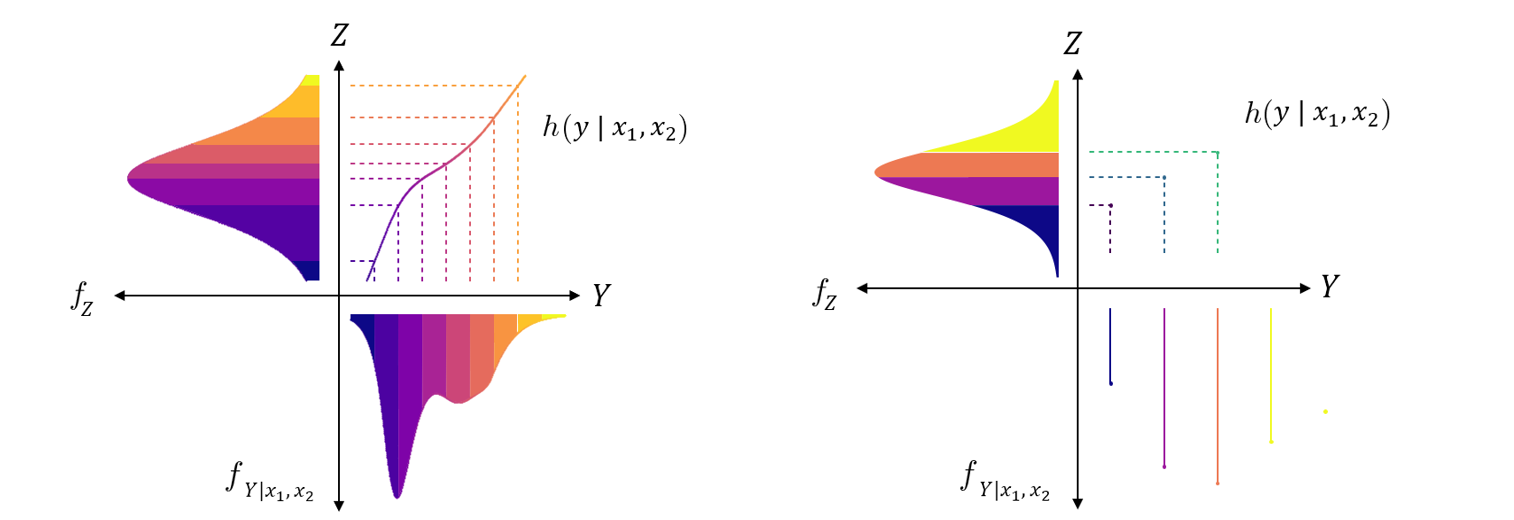
\includegraphics[width=1\textwidth]{img/tram_cont_ord.png}
\caption{Left: Example of a transformation model for a continuous outcome $Y$ with a smooth transformation function. Right: Example of a transformation model for an ordinal outcome $Y$ with 4 levels. The transformation function consists of cut-points separating the levels of the outcome.
In both cases the latent distribution $Z$ is the standard logistic and the predictors $\mathbf{x}$ induce a linear (vertical) shift of the transformation function.}
\label{fig:tram_cont_ord}
\end{figure}


The parameters $\boldsymbol{\beta}$ and $\boldsymbol{\vartheta}$ are estimated by minimizing the negative log-likelihood (NLL), defined as:


\begin{equation}
\text{NLL} = - \frac{1}{n} \sum_{i=1}^{n} \log \left(f_{Y \mid \mathbf{X} = \mathbf{x}}(y_i)\right),
\label{eq:nll_tram}
\end{equation}

where $f_{Y \mid \mathbf{X} = \mathbf{x}}(y_i)$ is the conditional density function of the outcome $Y$ given the predictors $\mathbf{x}$ of the $i$-th observation under the current parameterization. A full derivation is provided in Appendix \ref{sec:nll}.

Throughout this thesis, these transformation models form the foundation for estimating conditional distributions of variables within the TRAM-DAG framework. Unless stated otherwise, the latent distribution $F_Z$ is chosen to be the standard logistic, resulting in a logistic transformation model.



\subsection{Deep TRAMs} \label{sec:deep_trams}

The transformation models introduced earlier were extended into deep TRAMs using a modular neural network architecture \citep{sick2020}. The goal is to obtain a parameterized transformation function of the form

\begin{equation}
h(y \mid \mathbf{x}_L, \mathbf{x}_C ) = h_I(y) + \mathbf{x}_L^\top \boldsymbol{\beta} + f(\mathbf{x}_C),
\label{eq:deep_tram_old}
\end{equation}

where $h_I(y)$ is the intercept (simple or complex), $\mathbf{x}_{L}$ are predictors with a linear effect on the transformation function, and $\mathbf{x}_{C}$ are those with a potentially complex, non-linear influence. The parameters for each component of the model -- intercept, linear shift, and complex shift -- are obtained by a neural network module. The user can assign predictors to these components depending on the assumed structure of the data and the desired flexibility. Figure~\ref{fig:deep_tram} illustrates an example of a transformation function with these tree components (SI-LS-CS). For simplicity, it shows the simple intercept (SI) case where the intercept does not depend on predictors.


\begin{figure}[H]
\centering
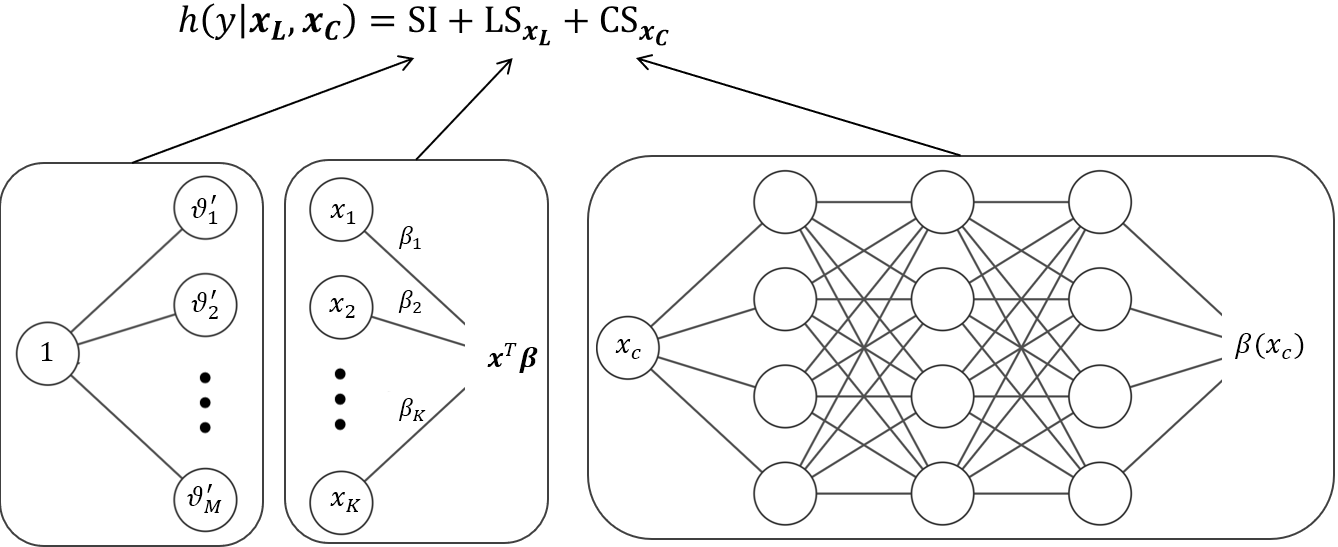
\includegraphics[width=0.9\textwidth]{img/deep_tram.png}
\caption{Modular deep transformation model (deep TRAM). The transformation function $h(y \mid \mathbf{x})$ is constructed from the outputs of three neural networks: intercept (SI/CI), linear shift (LS), and complex shift (CS). The intercept module (left) shows the simple intercept (SI) case and could be extended to a complex intercept (CI) by feeding predictors into the module and adding hidden layers and nonlinear activation functions.}
\label{fig:deep_tram}
\end{figure}

\medskip


\textbf{Intercept:} The intercept defines the baseline shape of the transformation function when $\mathbf{x}_{L}^\top \boldsymbol{\beta} = 0$ and $f(\mathbf{x}_{C}) = 0$. For continuous outcomes, it is modeled using a smooth Bernstein polynomial (Equation~\ref{eq:methods_bernstein_polynomial}), and for discrete outcomes via cut-points. The preliminary parameters $\tilde{\vartheta}_k$ are the output nodes of a neural network, and subsequently transformed to be monotonically increasing $\vartheta_k$. A simple intercept (SI) assumes no dependency on predictors and uses only a constant input. A complex intercept (CI), by contrast, allows the parameters to vary as a function of selected predictors by feeding $\mathbf{x}$ into a neural network with hidden layers, producing predictor dependent parameters $\vartheta_k(\mathbf{x})$. This allows the baseline distribution to adapt flexibly to different covariate settings. Details on the computation of the Bernstein polynomial are provided in Appendix~\ref{sec:bernstein_polynomial}.

\medskip

\textbf{Linear shift:} Predictors with an assumed linear influence on the transformation funciton are modeled via the linear shift (LS) component. Here, a neural network without hidden layers and without bias nodes receives $\mathbf{x}_{L}$ as input and returns a linear combination $\mathbf{x}_{L}^\top \boldsymbol{\beta}$ as output. This results in a vertical, linear shift of the transformation function. The parameters $\boldsymbol{\beta}$ are interpretable coefficients, and in the case of a logistic transformation model, represent log-odds ratios. See Appendix~\ref{sec:interpretation_linear_coefficients} for more details.

\medskip

\textbf{Complex shift:} Non-linear dependencies between predictors and the transformation function can be modeled by the complex shift (CS) component. The corresponding predictors $\mathbf{x}_{C}$ are input into a deep neural network (with at least one hidden layer and non-linear activation functions), yielding a scalar output $f(\mathbf{x}_{C})$. This allows modeling of non-linear predictor effects, including interactions between predictors if input multiple predictors into the neural network module. See Appendix~\ref{sec:complex_shift} for an example of modeling an interaction with a complex shift for the purpose of estimating individualized treatment effects (ITEs).

\medskip

\textbf{Level of complexity:} A key advantage of the deep TRAM architecture is that users can specify the role of each predictor: linear (LS), complex (CS), or influencing the shape of the transformation function (CI). For example, \citet{herzog2023} predicted the ordinal functional outcome three months after stroke by combining structured tabular data with image features (via a CNN) as predictors. This flexible design allows the integration of different data modalities into a single model.


\medskip

The resulting distribution function of deep TRAMs is invariant to the choice of the inverse-link function $F_Z$ (latent distribution) in an unconditional \citep{hothorn2018} or fully flexible (CI) setting. However, once restrictions are introduced on the influence of the predictors -- such as LS or CS -- the model assumes a fixed scale of dependence. The choice of latent distribution may depend on (i) assumptions about the data-generating process, (ii) the conventional and widely used interpretation scale for parameters (e.g., log-odds ratios for discrete outcomes or log-hazard ratios in survival analysis), and (iii) a data-driven criterion such as selecting the distribution that minimizes the negative log-likelihood (NLL) on the observed data.

%
\medskip

\textbf{Parameter estimation:} The weights of the neural networks are learned by minimizing the NLL of the conditional model. Starting from random weight initialization, the networks are trained using the Adam optimizer \citep{kingma2015}. Outputs of the modules are assembled to compute the NLL, and backpropagation \citep{rumelhart1986} is used to adjust weights iteratively. Deep learning techniques such as dropout \citep{srivastava2014}, early stopping \citep{prechelt2012}, and batch normalization \citep{Ioffe2015} can be applied to prevent overfitting and improve generalization. Nonlinear activation functions (e.g., ReLU \citealp{glorot2011} or sigmoid \citealp{rumelhart1986}) are used in hidden layers to capture complex relationships. \citet{schmidhuber2015} provides an extensive historical overview of deep learning methods and their development.




\subsection{TRAM-DAGs: Deep TRAMS applied in a causal setting} \label{sec:tram_dags}



In TRAM-DAGs, deep transformation models are applied within a causal setting. We assume a pre-specified DAG that represents the causal dependencies among variables. 
Figure~\ref{fig:tram_dag} illustrates the basic idea using a simple DAG with three variables and no hidden confounders. Each node's conditional distribution is modeled using a deep TRAM given its parent variables in the DAG. The assumed influence of the parent variables must be specified as CI, LS or CS. In this example, $X_1$ is a continuous source node (i.e., without parents) and its transformation function consists only of a simple intercept (SI). $X_2$ is also continuous and depends on $X_1$ by a linear shift (LS). $X_3$ is an ordinal variable with four levels; its transformation function is influenced linearly by $X_1$ (LS) and non-linearly by $X_2$ (CS). The cut-points $h(x_{3,k} \mid x_1, x_2)$ represent the cumulative log-odds of levels $k = 1, 2, 3$ of $X_3$. The probability of the highest category ($k = 4$) is the complement of the cumulative probability of the first three.


% include image /img/tram_dag.png
\begin{figure}[H]
\centering
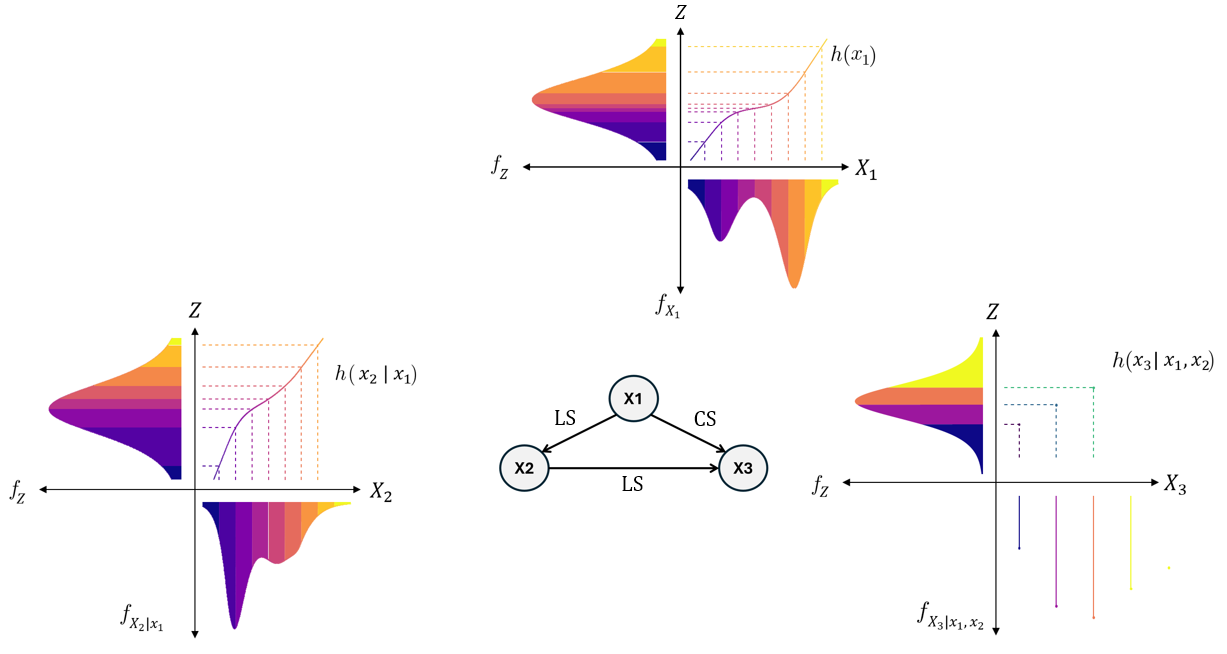
\includegraphics[width=0.95\textwidth]{img/tram_dag.png}
\caption{Example of a TRAM-DAG with three variables: $X_1$, $X_2$, and $X_3$. Each variable's distribution is modeled conditionally on its parents using deep TRAMs. Arrows indicate the causal dependencies.}
\label{fig:tram_dag}
\end{figure}

This DAG, along with its assumed dependencies, can be represented by a meta-adjacency matrix (Equation~\ref{eq:MA}), where rows indicate sources and columns indicate targets of causal influence:


\begin{equation}
\mathbf{MA} =
\begin{bmatrix}
  0 & \text{LS} & \text{LS} \\
  0 & 0  & \text{CS} \\
  0 & 0  & 0
\end{bmatrix}
\label{eq:MA}
\end{equation}

Based on this DAG, each variable's conditional distribution is modeled using a deep TRAM, enabling generative sampling and causal inference. The corresponding conditional distributions are:

\[
\begin{aligned}
X_1 &\sim F_Z(h_I(x_1)) \\
X_2 &\sim F_Z(h_I(x_2) + \mathrm{LS}_{x_1}) \\
X_3 &\sim F_Z(h_I(x_3) + \mathrm{LS}_{x_1} + \mathrm{CS}_{x_2})
\end{aligned}
\]

%
\textbf{Constructing the modular neural network:} As described in Section~\ref{sec:deep_trams}, the transformation functions are implemented using a modular neural network. The network takes as input the observed variables $\mathbf{x}$ and the meta-adjacency matrix~\ref{eq:MA}, which encodes the assumed causal structure. This matrix acts as a binary mask that restricts information flow to follow the directed edges of the graph, ensuring that only causal parent-to-child relationships are modeled. As a result, spurious dependencies such as $X_2 \rightarrow X_1$ are prevented. This masking approach is inspired by the Masked Autoregressive Flow (MAF) framework \citep{papamakarios2017}, where connectivity within the network is masked to control which inputs each output can depend on.

Before training the model, the input data must be appropriately preprocessed. Discrete variables with few categories are dummy encoded, and continuous variables should be scaled prior to input. Further discussion of encoding and scaling is provided in Appendix~\ref{sec:encoding_discrete_variables} and~\ref{sec:scaling_continuous_variables}.

Once the data are preprocessed and the structure is specified, the architecture of the neural networks for the complex shift or complex intercept must be defined -- including choices such as depth, width, activation functions, and whether to use dropout or batch normalization. These decisions depend on the assumed complexity of the effects and the need to regularize against overfitting.

Each node's transformation function is assembled from the outputs of its three modular components: the intercept (SI or CI), linear shift (LS), and complex shift (CS). Model training is performed by minimizing the NLL, optimizing all parameters at the same time. The estimated parameters $\boldsymbol{\beta}$ in the linear shift are interpretable as log-odds ratios corresponding to a one-unit increase in the respective parent variable, holding all other parent variables unchanged.




\subsection{Sampling from TRAM-DAGs} \label{methods:sampling}

Once a TRAM-DAG is fitted on data, it can be used to sample from the observational or interventional distribution, or to perform counterfactual queries. The structural equations $X_i = f(Z_i, \text{pa}(X_i))$ are represented by the inverse of the conditional transformation functions, i.e., $X_i = h^{-1}(Z_i \mid \text{pa}(X_i))$, since the transformation function maps from observed values to the latent scale: $Z_i = h(X_i \mid \text{pa}(X_i))$.


\medskip

\textbf{Observational sampling:} The sampling process from the observational distribution is described in Algorithm~\ref{alg:sampling} and illustrated in Figure~\ref{fig:sampling}. In each iteration, one complete sample of all variables in the DAG is generated -- i.e. a sample from the joint observational distribution.

\begin{algorithm}
\caption{Generate a complete sample from the observational distribution}
\label{alg:sampling}
\begin{algorithmic}
\State \textbf{Given:} A fitted TRAM-DAG with structural equations $X_i = h^{-1}(Z_i \mid \text{pa}(X_i))$
\For{each node $X_i$ in topological order}
  \State Sample latent value $z_i \sim F_{Z_i}$ \Comment{e.g., \texttt{rlogis()} in R}
  \If{$X_i$ is continuous}
    \State Solve $h(x_i \mid \text{pa}(x_i)) - z_i = 0$ for $x_i$ \Comment{numerical root-finding}
  \ElsIf{$X_i$ is discrete}
    \State Find category $x_i = \max \left( \{0\} \cup \left\{ x : z_i > h(x \mid \text{pa}(x_i)) \right\} \right) + 1
$
  \EndIf
\EndFor
\end{algorithmic}
\end{algorithm}


\begin{figure}[H]  % before [H]
\centering
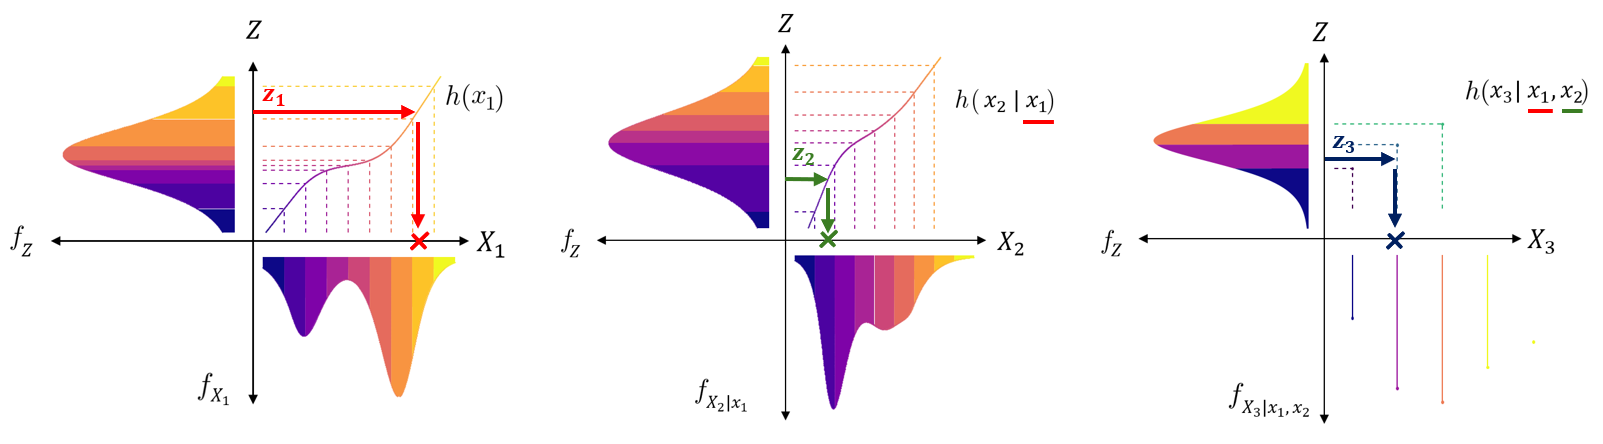
\includegraphics[width=1\textwidth]{img/sampling.png}
\caption{One sampling iteration for the three variables from the estimated transformation functions $h(x_i \mid \text{pa}(x_i))$. The latent values $z_i$ are sampled from the standard logistic distribution. The values $x_i$ are determined by applying the inverse of the transformation function for continuous variables or by finding the corresponding category for the ordinal variable. See Algorithm~\ref{alg:sampling} for details.}
\label{fig:sampling}
\end{figure}


% \textbf{Interventional sampling:} To sample from the interventional distribution, we can apply the do-operator as described by \citet{pearl1995} (though, Pearl named it set instead of do). The do-operator fixes a variable at a certain value. Hence, one can sample from the distribution of the other variables while keeping the fixed variable constant. For example, if one wants to intervene on $X_2$ and set it to a specific value $\alpha$, $\textcolor{red}{\text{do}(x_2 = \alpha})$
% and then sample from the interventional-distribution
% \[
% x_3 = \min \left\{ x : z_3 \le h(x \mid x_1, \textcolor{red}{x_2 = \alpha}) \right\}
% \]
% 
% with the same process as for the observational sampling, with the only difference that the intervened variable $X_2$ stays constant.


%  do-operator (originally referred to as "set")

\textbf{Interventional sampling:} To sample from an interventional distribution, we apply the \textit{do}-operator as described by \citet{pearl1995}. The \textit{do}-operator fixes a variable at a specific value, thereby removing its causal dependencies. This allows to simulate interventions by holding that variable constant while sampling the remaining variables as described earlier in Algorithm~\ref{alg:sampling}. For example, suppose we intervene on $X_2$ and set it to a specific value $\alpha$, denoted as $\text{do}(X_2 = \alpha)$. To sample from the resulting interventional distribution, we proceed as in observational sampling, with the only difference that $X_2$ is no longer sampled but fixed to the value $\alpha$. $X_1$ would not be affected by the intervention, as it is not a descendant of $X_2$ in the DAG. Therefore, sampling $X_3$ under this intervention would follow:

\[
x_3 = \max \left( \{0\} \cup \left\{ x : z_3 > h(x \mid x_1, \textcolor{red}{x_2 = \alpha}) \right\} \right) + 1.
\]


\textbf{Counterfactual queries:} In a counterfactual query, we are interested in what the value of a variable $X_i$ would have been, had another variable $X_j$ taken a different value than actually observed. \citet{pearl_book2009} describes a three-step procedure to answer such queries. In short, let $\mathbf{x}$ denote the observed values (a sample) of all variables in a DAG and let $\mathbf{z}$ denote the corresponding latent variables inferred via the transformation functions: $z_k = h_k(x_k \mid \text{pa}(x_k))$. Then, in a counterfactual query where $X_j$ is set to a new value $\alpha$ (intervention), we retain the same latent values $\mathbf{z}$, but apply the transformation functions in a post-interventional DAG with $X_j := \alpha$ to compute the counterfactual outcomes for the remaining variables.
The counterfactual estimation procedure is outlined in Algorithm~\ref{alg:single_cf} and visualized in Figure~\ref{fig:cf_viz}. Note that this visualization is simplified to illustrate only one parent variable ($X_j$); in practice, the set of parents $\text{pa}(X_i)$ may include additional predictors.

\begin{algorithm}[!ht]
\caption{Answer a single counterfactual query}
\label{alg:single_cf}
\begin{algorithmic}
\State \textbf{Given:} A TRAM-DAG model with estimated structural equations $X_k = h_k^{-1}(Z_k \mid \text{pa}(X_k))$
\State \textbf{Input:} Observed sample $\mathbf{x}$, intervention $X_j := \alpha$
\vspace{0.3em}
\State \textbf{Step 1 (Abduction):} For each observed variable $x_k$, compute the corresponding latent value $z_k = h_k(x_k \mid \text{pa}(x_k))$
\vspace{0.3em}
\State \textbf{Step 2 (Action):} Modify the DAG by setting $X_j := \alpha$ (intervention)
\vspace{0.3em}
\State \textbf{Step 3 (Prediction):} Using the counterfactual DAG and the intervened value $X_j = \alpha$, go along the causal order and determine the counterfactual values for all descendants $X_k$ of $X_j$. This is done by evaluating
\[
x_k = h_k^{-1}(z_k \mid \text{pa}^*(x_k)),
\]
where $z_k$ is the latent value obtained in Step 1, and $\text{pa}^*(x_k)$ are the (possibly updated) parent values after the intervention.
\end{algorithmic}
\end{algorithm}

\begin{figure}[!ht]
\centering
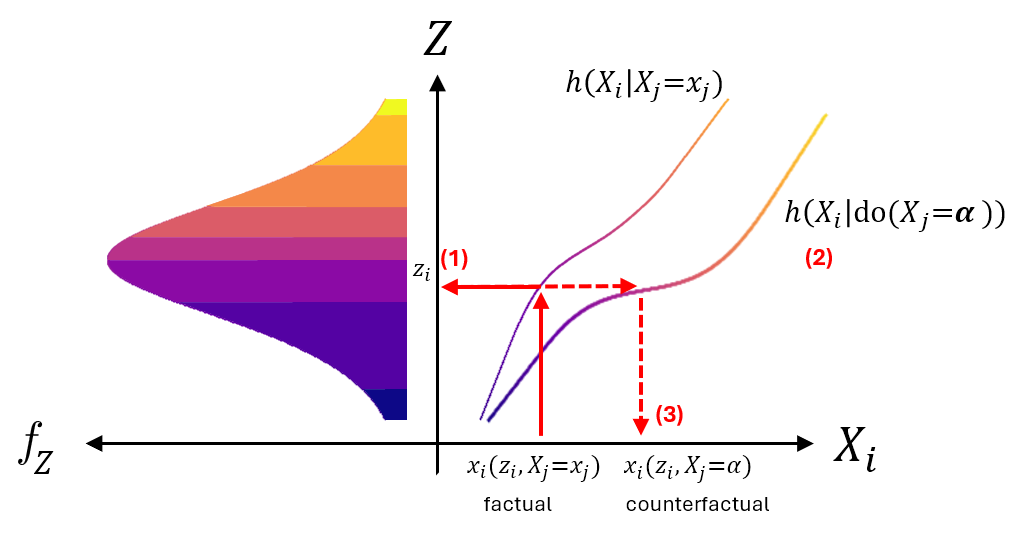
\includegraphics[width=0.65\textwidth]{img/counterfactuals.png}
\caption{Illustration of a counterfactual query for variable $X_i$, had its parent $X_j$ taken a different value, following the three-step procedure: (1) abduction of the latent value $z_i$ from the observed outcome, (2) intervention by setting $X_j = \alpha$, (3) prediction of the counterfactual outcome using the same $z_i$ and the modified transformation function. This simplified example assumes a single parent variable; in practice, $\text{pa}(X_i)$ may include multiple predictors.}
\label{fig:cf_viz}
\end{figure}



While counterfactual probabilities (e.g., $P(X_i = x \mid \text{do}(X_j = \alpha), z_i)$) are well-defined in both continuous and discrete settings, determining the counterfactual realizations is generally only possible for continuous variables. In the discrete case, no unique latent value $z_k$ can be recovered from an observed category, as multiple $z_k$ values may map to the same outcome. Consequently, only the probabilities of counterfactual outcomes can be evaluated for discrete variables, not their exact values. This is a fundamental limitation of counterfactual reasoning in discrete settings with continuous latent variables.

% 
% \textbf{Counterfactual queries:} In a counterfactual query, we are interested in what the value of a variable $X_i$ would have been, had another variable $X_j$ taken a different value than it actually did. \citet{pearl_book2009} describes a three-step procedure to answer such queries. Given a structural causal model $M$ and observed evidence $e$ (i.e., the values of all variables $\mathbf{x}$ in one observed sample sample), the goal is to compute the counterfactual value or probability of $Y = y$ under the hypothetical condition $X = x$.
% 
% \vspace{1em}
% \noindent
% The three steps, known as \textbf{abduction}, \textbf{action}, and \textbf{prediction}, are:
% 
% \begin{itemize}
%     \item \textbf{Abduction:} With the model $M$ infer the latent variables $Z$ that explain the observed sample $x$.
%     \item \textbf{Action:} Modify the model $M$ by applying the intervention \( \text{do}(X_i = \alpha) \), i.e., set $X_j$ to the hypothetical value $\alpha$.
%     \item \textbf{Prediction:} Use the updated model and latent variables to compute the counterfactual value or distribution of $X_i$.
% \end{itemize}
% 
% \vspace{1em}
% \noindent
% This procedure is illustrated in Figure~\ref{fig:cf_illustration} and formalized in the pseudocode below.
% 
% % Insert your image for counterfactual here
% \begin{figure}[H]
% \centering
% \includegraphics[width=0.8\textwidth]{img/counterfactual.png}
% \caption{Illustration of the three steps in counterfactual reasoning.}
% \label{fig:cf_illustration}
% \end{figure}
% 
% \begin{algorithm}
% \caption{Answer a Single Counterfactual Query}
% \label{alg:single_cf}
% \begin{algorithmic}
% \State \textbf{Given:} A structural model \( X_k = f(Z_k, \text{pa}(X_k)) \), with inverse noise map \( Z_k = h(X_k \mid \text{pa}(X_k)) \)
% \State \textbf{Input:} Observed sample \( x \), intervention \( X_i := \alpha \), target variable \( X_j \)
% \vspace{0.5em}
% \State \textbf{Step 1: Abduction} \hspace{0.5em} Compute latent noise \( Z_j = h(x_j \mid \text{pa}(x_j)) \)
% \State \textbf{Step 2: Action} \hspace{1.6em} Replace \( x_i \) with \( \alpha \) in the parent set \( \text{pa}(X_j) \)
% \State \textbf{Step 3: Prediction} \hspace{0.3em} Compute \( x_j^{cf} = h_j^{-1}(Z_j \mid \text{pa}(X_j)^{cf}) \)
% \end{algorithmic}
% \end{algorithm}
% 
% \vspace{1em}
% \noindent
% While the \emph{distribution} of a counterfactual variable \( Y \) under a hypothetical intervention \( X = x \) can be estimated for both discrete and continuous outcomes, the \emph{actual counterfactual value} is only well-defined for continuous outcomes. For discrete variables, latent variables can be abduced, but the inverse map \( h^{-1} \) may not yield a unique category.
% 
% 
% \textbf{Counterfactual queries}: In a counterfactual query one wants to know what the value of variable $X_i$ would have been if another variable $X_j$ had a different value than what was actually observed. \citet{pearl_book2009} describes the three-step process to answer counterfacutal queries as follows: Given a causal model $M$ and observed evidence $e$ (which are the actually observed values of the variables $X_i$ of one sample) one wants to compute the probability of $Y=y$ under the hypothetical condition $X=x$.
% 
% 
% Here input image of counterfactuals from final presentation.
% 
% 
% Step 1 aims to explain the past (Z) by knowledge of the evidence e; 
% Step 2 amends the past to the hypothetical condition $X=x$ 
% Step 3 predicts the future (Y) based on our new understanding of the past and our newly established condition, $X =x$
% 
% Pearl named these three steps, (1) abduction,  (2) action and (3) prediction. The procedure is described in the pseudocode \ref{alg:counterfactual} and illustrated in Figure.
% 
% \begin{algorithm}
% \caption{Answer a Single Counterfactual Query}
% \label{alg:single_cf}
% \begin{algorithmic}[1]
% \State \textbf{Given:} A structural model $X_k = f(Z_k, \text{pa}(X_k))$, with inverse noise map $Z_k = h(X_k \mid \text{pa}(X_k))$
% \State \textbf{Input:} Observed sample $x$, intervention $X_i := \alpha$, target variable $X_j$
% \vspace{0.3em}
% \State \textbf{Step 1: Abduction} Infer latent variable $Z_j = h(x_j \mid \text{pa}(x_j))$ using the observed values
% \vspace{0.3em}
% \State \textbf{Step 2: Action} Replace the value of $X_i$ with $\alpha$ in the set of parent variables
% \vspace{0.3em}
% \State \textbf{Step 3: Prediction} Compute the counterfactual value $x_j^{cf} = h_j^{-1}(Z_j \mid \text{pa}(x_j)^{cf})$
% \vspace{0.3em}
% \end{algorithmic}
% \end{algorithm}
% 
% 
% 
% While the probability of Y under the hypothetical condition $X=x$ can be determined in any case, the actual counterfactual value of Y is only defined for a continuous outcome but not for discrete outcomes.

% see pearl book causality: 1.4.4 Counterfactuals in Functional Models (page 36)

% (What pearl writes:  Likewise, in contrast with the potential-outcome framework, counterfactuals in the structural account are not treated as undefined primitives but rather as quantities to be derived from the more fundamental concepts of causal mechanisms and their structure. )











% enforce that starts after all floats have been displayed
\FloatBarrier


\section{Individualized Treatment Effect (ITE)} \label{sec:methods_ite}



% - Short intro to individualized treatment effects and its importance, including that RCT's only measure ATE
% - definition of Individual treatment effect with formula, including potential outcomes (Rubin causal model /potential outcomes framework)
% - CATE and ITE are the same and are estimate of the individual effect
% - note that we will use ITE for simplicity but also CATE is meant
% - formula of ITE with Probabilities for a binary treatment and outcome 
% - Introduction of quantile treatment effects, just short with formula (same expept quantile instead expected value)
% - homogeneous vs. heterogeneous treatment effects (with interaction example, already hint that despite no interaction there can still be heterogeneous treatment effects, due to covariates and nonlinear transformation)
% 
% - Assumptions: identifiability (ignorability?)
% 
% - Models for ITE estimation: meta learners (T, S, X), virtual twins
% -calibration must be good, prevent overfitting
% 
% - validation techniques for ITE estimation: ITE densities, ITE-ATE plots, simulation scatterplots, ATE on average (Confidence intervals and bootstrapping better talked about in respective experiment methods), (if ITE are correct, they should be on average the ATE, but if it is the same we cannot say certailny that the ITE are correct)
% 
% 
% 
% --> explain in detail in the discussion the phenomenon of ghost interactions, 
%  and possible solutions (IV, )




% https://ascpt.onlinelibrary.wiley.com/doi/epdf/10.1002/cpt.3159
% --> perfect introduction and overview and assumptions also in observatinoal setting about ITE with causal ML --> check it!
% also limitations and how to validate models

% Check Hooglands paper (guide) again, he should also say something about benefits of RCT that might be relevant for my subjects.

% https://arxiv.org/pdf/2108.04939
% above paper also discusses the implications of strong identifiability assumpions and that cate still can be biased if there are unobserved interaction variables. (however, not sure how good this paper is, many typos)


RCTs are considered the gold standard for estimating the causal effect of a treatment due to their ability to eliminate confounding through randomization \citep{little2000}. However, RCTs typically aim to estimate the average treatment effect (ATE), which summarizes the effect of the treatment across the entire study population. This approach overlooks individual-level variation in treatment response: depending on their unique characteristics, some individuals may benefit substantially, others not at all, or even be harmed. While the homogeneous treatment effect refers to the part of the effect that is equal for all patients, the heterogeneous treatment effect (HTE) describes the variation in treatment effects across individuals or subgroups. One reason for treatment effect heterogeneity is the presence of interaction variables \citep{hoogland2021}, also referred to as effect modifiers \citep{christensen2021}, which influence how the treatment effect varies depending on individual characteristics. However, even in the absence of explicit interaction variables, treatment effects can still exhibit heterogeneity due to the scale on which personalized effects are evaluated \citep{hoogland2021}. This phenomenon is further explored in Experiment 4 and will be discussed in detail in Section~\ref{sec:disc_experiment4}.

In personalized medicine and informed decision-making, individual-level treatment effects are more relevant than population averages. The individual treatment effect compares the potential outcomes for an individual~$i$ under two different treatment options: the potential outcome $Y_i(1)$ under treatment, and $Y_i(0)$ under control, as defined by Rubin's potential outcomes framework~\citep{rubin2005}. The individual treatment effect is typically defined as the difference between the two potential outcomes:


\begin{equation}
Y_i(1) - Y_i(0).
\end{equation}



However, for any individual, only one of these two potential outcomes can be observed -- the other one remains counterfactual. This is known as the fundamental problem of causal inference \citep{holland1986}, and it implies that the individual treatment effect is inherently unobservable. To estimate causal effects from observed data, several assumptions must be made to ensure identifiability.

\medskip 

\textbf{Assumptions for Identifiability:} Unlike standard predictive modeling, the estimation of causal effects requires untestable assumptions to link observed data with unobserved counterfactuals. A central assumption is consistency, which requires that the observed outcome equals the potential outcome under the treatment actually received: $Y = Y(1)$ if $T = 1$, and $Y = Y(0)$ if $T = 0$. The Stable Unit Treatment Value Assumption (SUTVA) assumes no interference between units and that treatments are well-defined \citep{rubin1980}. The most critical assumption is ignorability (or unconfoundedness), which states that, conditional on observed covariates $X$, the treatment assignment is independent of the potential outcomes \citep{rosenbaum1983}:

\begin{equation}
(Y(1), Y(0)) \perp T \mid X.
\end{equation}

This implies that there are no unmeasured confounders affecting both treatment assignment and outcomes. In an RCT, this condition is typically satisfied by design. In contrast, for observational data, all relevant confounders must be measured and conditioned on. Additionally, the positivity assumption requires that every individual has a non-zero probability of receiving each treatment level:

\begin{equation}
0 < P(T = 1 \mid X = x) < 1 \quad \text{for all } x.
\end{equation}

\medskip

While the individual treatment effect is inherently unobservable, its expectation conditional on covariates can be identified under the assumptions above. This quantity is referred to as the conditional average treatment effect (CATE), or individualized treatment effect (ITE). In this thesis, we use the term ITE to denote this estimand. For an individual with covariates \( \mathbf{X}_i = \mathbf{x}_i \), the ITE can be identified as:

\medskip



\begin{align}
\text{ITE}_i(\mathbf{x}_i) &= \mathbb{E}[Y_i(1) - Y_i(0) \mid \mathbf{X}_i = \mathbf{x}_i] \notag \\[0.5em]
&= \mathbb{E}[Y_i(1) \mid \mathbf{X}_i = \mathbf{x}_i] - \mathbb{E}[Y_i(0) \mid \mathbf{X}_i = \mathbf{x}_i] \notag \\[0.5em]
&= \mathbb{E}[Y_i(1) \mid T_i = 1, \mathbf{X}_i = \mathbf{x}_i] 
 - \mathbb{E}[Y_i(0) \mid T_i = 0, \mathbf{X}_i = \mathbf{x}_i] \quad \text{(by ignorability)} \notag \\[0.5em]
&= \mathbb{E}[Y_i \mid T_i = 1, \mathbf{X}_i = \mathbf{x}_i] 
 - \mathbb{E}[Y_i \mid T_i = 0, \mathbf{X}_i = \mathbf{x}_i] \quad \text{(by consistency)}
\end{align}



% 
% \begin{equation}
% \text{ITE}_i(\mathbf{x}_i) = \mathbb{E}[Y_i(1) - Y_i(0) \mid \mathbf{X}_i = \mathbf{x}_i] 
% = \mathbb{E}[Y_i(1)\mid \mathbf{X}_i = \mathbf{x}_i] - \mathbb{E}[Y_i(0)\mid \mathbf{X}_i = \mathbf{x}_i]
% \end{equation}
% 
% It reflects the expected, or average, treatment effect for an individual~$i$, conditional on that individual's specific covariates~$\mathbf{X}_i = \mathbf{x}_i$.
% 
% 
% \noindent
% Under the assumption of \textbf{ignorability} (also called unconfoundedness), that is, $(Y_i(1), Y_i(0)) \perp T_i \mid \mathbf{X}_i$, the expression can be rewritten as:
% 
% \begin{equation}
% \text{ITE}_i(\mathbf{x}_i) = \mathbb{E}[Y_i(1) \mid T_i = 1, \mathbf{X}_i = \mathbf{x}_i] 
% - \mathbb{E}[Y_i(0) \mid T_i = 0, \mathbf{X}_i = \mathbf{x}_i]
% \end{equation}
% 
% \medskip
% 
% \noindent
% Finally, under the \textbf{consistency} assumption, we can substitute $Y_i = Y_i(1)$ and $ Y_i = Y_i(0)$:
% 
% \begin{equation}
% \text{ITE}_i(\mathbf{x}_i) = \mathbb{E}[Y_i \mid T_i = 1, \mathbf{X}_i = \mathbf{x}_i] 
% - \mathbb{E}[Y_i \mid T_i = 0, \mathbf{X}_i = \mathbf{x}_i]
% \end{equation}

\medskip

In the case of a binary outcome $Y$, where the expected value corresponds to the probability that $Y = 1$, the ITE for an individual with covariates $\mathbf{X}_i = \mathbf{x}_i$, under the identifiability assumptions, is given by:

\medskip

\begin{equation}
\text{ITE}_i(\mathbf{x}_i) = P(Y_i = 1 \mid T_i = 1, \mathbf{X}_i = \mathbf{x}_i) - P(Y_i = 1 \mid T_i = 0, \mathbf{X}_i = \mathbf{x}_i).
\end{equation}

\medskip

If $Y = 1$ indicates recovery, a positive ITE means that the individual is expected to benefit from the treatment compared to control. A negative ITE suggests a lower probability of recovery under treatment, while an ITE of zero indicates no expected difference between treatment and control for that individual.



\medskip




% 
% RCTs are considered the gold standard for estimating the causal effect of a treatment due to their ability to eliminate confounding through randomization \citep{little2000}. However, RCTs typically aim to estimate the average treatment effect (ATE), which summarizes the effect of the treatment across the entire study population. This approach overlooks individual-level variation in treatment response: depending on their unique characteristics, some individuals may benefit substantially, others not at all, or even be harmed. While the homogeneous treatment effect refers to the part of the effect that is equal for all patients, the heterogeneous treatment effect (HTE) describes the variation in treatment effects across individuals or subgroups. One reason for treatment effect heterogeneity is the presence of interaction variables \citep{hoogland2021}, also referred to as effect modifiers \citep{christensen2021}, which influence how the treatment effect varies depending on individual characteristics. However, even in the absence of explicit interaction variables, treatment effects can still exhibit heterogeneity due to the scale on which personalized effects are evaluated \citep{hoogland2021}. This phenomenon is further explored in Experiment 4 and will be discussed in detail in Section~\ref{sec:disc_experiment4}.
% 
% In personalized medicine and informed decision-making, individual-level treatment effects are more relevant than population averages. The individual treatment effect compares the potential outcomes for an individual~$i$ under two different treatment options: the potential outcome $Y_i(1)$ under treatment, and $Y_i(0)$ under control, as defined by Rubin's potential outcomes framework~\citep{rubin2005}. It is typically defined as the difference between the two potential outcomes:
% 
% 
% \begin{equation}
% Y_i(1) - Y_i(0).
% \end{equation}
% 
% 
% 
% However, only one of the two potential outcomes can be observed for each individual, which is known as the fundamental problem of causal inference~\citep{holland1986}. Instead, most methods aim to estimate the expected treatment effect conditional on a given set of covariates~$\mathbf{X}$. This quantity is known as the conditional average treatment effect (CATE), which is valid under assumptions discussed later:
% 
% 
% \begin{align}
% \text{CATE}_i(\mathbf{x}_i) &= \mathbb{E}[Y_i(1) - Y_i(0) \mid \mathbf{X}_i = \mathbf{x}_i] \notag \\
%                  &= \mathbb{E}[Y_i \mid T = 1, \mathbf{X}_i = \mathbf{x}_i] - \mathbb{E}[Y_i \mid T = 0, \mathbf{X}_i = \mathbf{x}_i]
% \end{align}
% 
% 
% It reflects the expected, or average, treatment effect for an individual~$i$, conditional on that individual's specific covariates~$\mathbf{X}_i = \mathbf{x}_i$.
% 
% In fields such as healthcare, the CATE is often referred to as the individualized treatment effect (ITE), as for example done by~\citet{hoogland2021}. In this thesis, we use the term ITE to denote individualized treatment effects, i.e., CATE.
% 
% The ITE for an individual with covariates $\mathbf{X}_i = \mathbf{x}_i$ in the case of a binary outcome and binary treatment is defined as:
% 
% \begin{equation}
% \text{ITE}_i(\mathbf{x}_i) = P(Y_i = 1 \mid T = 1, \mathbf{X}_i = \mathbf{x}_i) - P(Y_i = 1 \mid T = 0, \mathbf{X}_i = \mathbf{x}_i).
% \end{equation}
% 
% Assuming $Y = 1$ indicates recovery, a positive ITE means the individual is expected to benefit from the treatment compared to control. A negative ITE suggests the outcome is expected to be worse under treatment, while an ITE of zero implies no expected difference between treatment and control for that individual.
% 
% \medskip
% 
% \textbf{Assumptions for Identifiability:} Unlike standard predictive modeling, the estimation of the individualized treatment effect relies on untestable assumptions to ensure identifiability of causal effects from observational data. A central assumption is consistency, which requires that the observed outcome equals the potential outcome under the received treatment: $Y = Y(1)$ if $T = 1$, and $Y = Y(0)$ if $T = 0$. The Stable Unit Treatment Value Assumption (SUTVA) assumes no interference between units and that treatments are well-defined \citep{rubin1980}. The most critical assumption is ignorability (or unconfoundedness), which states that, conditional on observed covariates $X$, the treatment assignment is independent of the potential outcomes \citep{rosenbaum1983}:
% 
% \begin{equation}
% (Y(1), Y(0)) \perp T \mid X.
% \end{equation}
% 
% This implies that there are no unmeasured confounders affecting both treatment and outcome. Additionally, the positivity assumption requires that every individual has a non-zero probability of receiving each treatment level:
% 
% \begin{equation}
% 0 < P(T = 1 \mid X = x) < 1 \quad \text{for all } x.
% \end{equation}
% 
% 
% \medskip
% 

% An example of ITE estimation using a TRAM-DAG is provided in Appendix~\ref{appendix:ite_tram_example}.


\textbf{Models for ITE Estimation:} \label{sec:ite_models} A variety of methods exist to estimate ITEs. In this thesis, we focus on metalearners, specifically the T-learner and S-learner frameworks \citep{kunzel2019}. These methods are model-agnostic, meaning that any predictive algorithm can be used as a base model. There exists a variety of other approaches to model ITEs. The T-learner fits two separate models: one on the treated group and on the control group. The ITE for an individual is then estimated as the difference between the predicted outcomes from these two models. In contrast, the S-learner fits a single model on all individuals, incorporating the treatment indicator as an additional covariate to distinguish between treatment conditions. Therefore, the S-learner requires a model that is complex enough, to capture interaction effects between treatment and covariates. The experiments in this thesis were conducted using S- and T-learners that were based on TRAM-DAGs, logistic regression, logistic lasso regression, and random forests. Applied as S-learners, TRAM-DAGs with complex shift or intercept terms allow for flexible modeling of treatment effect heterogeneity. 

Accurate ITE estimation requires models that generalize well. Since ITEs are computed as differences between two outcome predictions, even small errors can accumulate. \citet{hoogland2021} emphasize the need to balance model complexity with data availability to avoid overfitting. They also highlight that estimating risk differences is inherently more challenging than predicting single outcomes. Furthermore, calibration is crucial when ITEs are derived from predicted potential outcomes \citep{hoogland2024}. While neural networks may be accurate, they often produce poorly calibrated probabilities \citep{guo2017}, which can mislead treatment effect estimation. Similarly, conventional models like logistic regression can overfit in small samples or high-dimensional settings, leading to extreme predictions. Penalization methods such as lasso shrink coefficients to improve generalization \citep{riley2021}, though studies have shown that they can perform inconsistently in low-sample scenarios \citep{calster2020}. These factors are important to consider when ITEs.
When using random forests as S-learners, care must be taken to ensure that the treatment variable is included in the splits. Proper tuning of hyperparameters like tree depth and variable selection (e.g., \texttt{mtry}) may be necessary to avoid overfitting.
In summary, model choice for ITE estimation should consider the complexity of treatment-outcome relationships, sample size, and calibration needs. While complex models like TRAM-DAGs and random forests can capture complicated heterogeneity, simpler models may offer more robust performance in smaller datasets or where treatment-covariate interactions are straightforward.



% 
% 
% A variety of methods are applied to estimate ITEs; in this thesis we focus on metalearners \citep{kunzel2019}, in particular S-learners and T-learner. S-learners use a single model that uses the treatment as covariate to predict both potential outcomes. T-learners fit two separate models, one on each treatment group. These two methods are model agnostic, hence any type of model can be used. In this thesis follwoing models were applied: TRAM-DAGs, logistic regression, lasso regression, and random forests.
% 
% \citet{hoogland2021} highlighted the importance of considering the model complexity and the susceptibility to overfitting. For ITE estimation, the models must generalize to a new sample. 
% The ITE for a binary endpoint is estimated as the difference of two probabilities (the risk under treatment minus the risk under control). It is essential that the model used to estimate these probabilities is well calibrated and generalizes to new (unseen) data. \citep{guo2017} point out that even though modern neural networks became much more accurate in terms of prediction performance, they are no longer well-calibrated. As it may not be a big problem for the sole purpose of making good predictions, it is very problematic for applications where an accurate quantification of the uncertainty is needed. When using models that are estimated with conventional methods such as ordinary least squares or standard maximum likelihood, they tend to overfit on the training data and make too extreme predictions on the test data. This problem increases with reduced sample size, low event rate or large number of predictor variables. To prevent such overfitting in regression models, penalization (shrinkage) methods are proposed as they shrink the estimated coefficients towards zero to reduce the variance in predictions on new data \citep{riley2021}. 
% 
% 
% \citet{curth2024} provide a comprehensive overview of the individualized treatment effect (ITE) and its estimation in the context of causal machine learning. They state its importance in comparison to average treatment effects, the assumpitons that need to be fulfilled, what kind of limiations typically are encountered and how models should be validated.

% take this paper as guide to the structure of this section to explain overview and concept
% https://ascpt.onlinelibrary.wiley.com/doi/epdf/10.1002/cpt.3159

% another paper of Alicia Curth https://proceedings.mlr.press/v130/curth21a/curth21a.pdf



% https://pmc.ncbi.nlm.nih.gov/articles/PMC5074325/ explained how to calibrate random forests for probability estimation (or just explain what comets does, maybe enough)


% Logistic regression, penalized logistic regression (shrinkage, lasso
% Shrinkage methods should provide better predictive perfomance on average (cite articles). \citet{calster2020} analyzed different regression shrinkage methods with a binary outcome in a simulation study. They concluded, although the calibration slope improved on average, shrinkage often worked poorly on individual datasets. With small sample size and low number of events per variable the performance of most of these methods were highly variable and should be used with caution in such settings. \citet{riley2021} obtained to similar results in their simulation study. Problems occur, because tuning parameters are often estimated with large uncertainty on the training data and fail to generalize. In both studies the autors pointed out that these penalization methods are more unreliable when needed most, that is when the risk of overfitting may be large.
% 
% When using a Random Forest based method as an S-learner (where Treatment is given as input variable) one has to make sure that the treatment variable is really used in the forests and not left out by mtry (not all variables are used for splits because decorrelating and reducing overfit.)
% 
% (Shrinkage shrinks the coefficients so that the calibration slope is improved on a test set. The shrinkage factor can for example be found with n-fold cross validation, as e.g. done by lasso with L1 penalization)
% 
% Explain tuning of random forest, with depth number of trees and mtry
% 
% TRAM-DAGs with complex shifts or compmlex intercepts can capture heterogeneity. See appendix XXX for an example of ITE estimation with a complex shift.



% Explain the kinds of validation measures & plots so that i dont have to explain them again in the next sections (experiments)


\medskip

\textbf{Validation of ITE Estimation:} \label{sec:ite_validation} \citet{hoogland2024} examined a variety of evaluation methods for assessing discrimination and calibration in ITE estimation. They emphasize that accurate prediction of potential outcomes should be considered a prerequisite for reliable ITE modeling. Furthermore, as in standard prediction modeling, proper validation should ideally be performed on independent (out-of-sample) data.
In this thesis, although various quantitative evaluation metrics exist, we primarily relied on visual validation tools. One such approach is the ITE-ATE plot, where individuals are grouped based on their predicted ITEs. Within each ITE-subgroup, the empirical ATE is calculated using observed outcomes. If the ITE estimates are well-calibrated, the observed ATEs should align the predicted values, resulting in a calibration curve that lies along the identity line. Additionally, in simulation experiments where the true ITEs are known, estimation accuracy was assessed by directly comparing predicted and true effects. Furthermore, model calibration in terms of predictive performance $P(Y \mid \mathbf{X} = \mathbf{x})$ was evaluated using calibration plots. As an additional check, the average of the estimated ITEs across the population should equal the estimated ATE, i.e., $\mathbb{E}[\text{ITE}(X)] = \text{ATE}$. Large deviations from this condition may indicate systematic bias. However, satisfying this equality does not guarantee that the estimated ITEs are accurate at the individual level. All evaluations were conducted both on the training data and on a separate hold-out test set.

% It should be noted, that when estimating the ITEs , the mean of the ITEs across the population should equal the ATE, i.e., $\mathbb{E}[\tau(X)] = \text{ATE}$. However, if one estimated ITEs whose average is equal to the ATE in a population, this does not neccesarily mean that the estimated ITEs are correct. 
% 
% See \citep{hoogland2024} for a analyzis of ITE estimation validation methods. He mentions it is best to check out of sample. 
% 
% In this thesis we rely mostly on visual validation tools such as ITE-ATE plots where individuals are grouped according to the predicted ITE and in each ITE subgroup the ATE is computed according to the actually observed outcomes. If ITE estimation is correct, the ATE in each subgroup should be equal to the predicted ITE, hence exhibit a calibration line on the identity line. Furthermore, in the experiments based on simulations, the true ITE is known, which allows to compare the estimated ITEs with the true ITEs. 
% 



% Assessing predictive performance with AUC, calibration slope, and brier score. In Leo presentation, he says that recalibration can either be done with deviance statistics or by leave one out (loo) cross validation the slope of this regression would then be the estimated shrinkage factor.




% If ITEs are correct, they should give on average the ATE: E(ITE) = ATE, (cite a paper, maybe Alicia Curth or Hoogland?). However, we can not say that the ITEs must be correct, if they give the ATE on average. (because they could for example also be much more spread than the true ITEs but still give the correct ATE on average!)







%%%%%%%%%%%%%%%%%%%%%%%%%%%%%%%%%%%%%%%%%%%%%%%%%%%%%%%%%%%%%%%%%%%%%%%%%%%%%%%%%%%%%%%%%%%%%%%%%%%%%%%%%%%%%%%%%%


% - also talk about propensity score Rubin(2007) to basically estimate an RCT...and overcome the problem of confounding. but this might work for ATE but not really for ITE, direct modelling of the outcome is necessary % https://pmc.ncbi.nlm.nih.gov/articles/PMC5920646/


% https://journals.sagepub.com/doi/pdf/10.1177/1536867X1001000309 also explain how to do quantile treatment effect QTE estimation with instrumental variables etc



% In this thesis , I will apply Lasso regression on the IST stroke trial and simulation studies, where the sample size is relatively large.


% simulation studies
%  "The setup was such that development and test sets were generated from the same data generating mechanism. In practice, there may be differences between these two settings that are not captured by the models, and the uncertainty that accompanies these unknowns may overshadow relatively small gains realized by more complex models."
%  % https://pmc.ncbi.nlm.nih.gov/articles/PMC9291969/#sim9154-bib-0065
 
 % "This could include the analysis of individual patient data from multiple randomized trials, or even the use of nonrandomized studies for the estimation of outcome risk under a control condition." this motivates the need for observational modeling.


% Problems with ITE: (in an RCT setting)
% - to estimate the ITE we must assume un-confoundedness. Does this also apply to itneractions (effect modifiers)? Check how this is handled in the literature.
% https://journals.lww.com/epidem/fulltext/2007/09000/four_types_of_effect_modification__a.6.aspx talks about different types of effect modifiers (not sure if this really contributes to the thesis)






% 
% 

% 
% 


% \subsection{Propensity Score Adjustment in Observational Settings}
% 
% In the absence of randomization, the \textit{propensity score}, defined as the probability of receiving treatment conditional on covariates $X$,
% \begin{equation}
% e(X) = P(T = 1 \mid X),
% \end{equation}
% can be used to balance treatment groups and reduce confounding rosenbaum1983central. When the ignorability assumption holds, adjusting for the propensity score allows for unbiased estimation of average treatment effects. However, while propensity score methods (e.g., matching, stratification, weighting) are effective for estimating population-level quantities like the ATE, they are often insufficient for ITE estimation. Since ITE requires modeling both potential outcomes at the individual level, direct modeling approaches such as outcome regression, meta-learners, or Bayesian models are typically more appropriate rubin2007design, nie2021quasi. Moreover, reliance on the propensity score alone may fail to capture fine-grained individual heterogeneity necessary for personalized treatment decisions ali2019addressing.






\section{Experiment 1: TRAM-DAG (simulation)} \label{sec:methods_experiment1}

This experiment demonstrates the application of TRAM-DAGs on a synthetic dataset, using the illustrative DAG previously shown in Figure~\ref{fig:tram_dag}. The objective is to show how TRAM-DAGs can learn structural equations from observational data by fitting a model to the joint distribution that resulted from the underlying causal structure.

We visualized the model fitting in terms of the training loss and subsequently showed and interpreted the learned components of the transformation functions, such as intercepts, linear and complex shifts. Finally, we drew samples from the estimated distributions to obtain observational and interventional distributions. We also conducted counterfactual queries on the learned model.

\medskip

\textbf{Data-generating process: } We simulated a dataset with three variables, $X_1$, $X_2$, and $X_3$, following the structure of the DAG and its associated meta-adjacency matrix shown in Figure~\ref{fig:dag_and_matrix}. The matrix describes the functional dependencies between variables, where LS indicates a linear shift and CS a complex shift. Rows represent the source of the effect, and columns the target.


\begin{figure}[H]
\centering
\begin{tikzpicture}[baseline={(current bounding box.center)}]
  \node (img) at (0, 0) {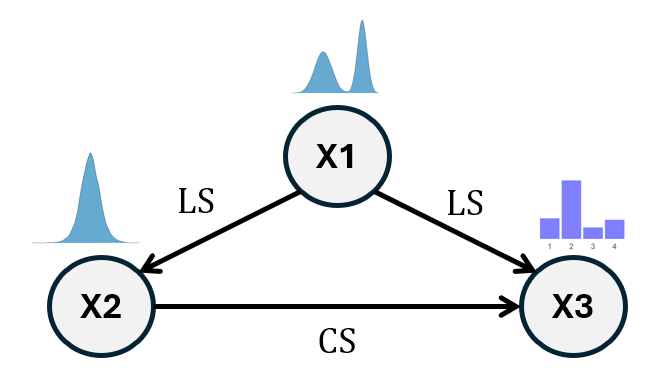
\includegraphics[width=0.28\textwidth]{img/exp1_DAG_MA.png}};
  \node (matrix) at (5, 0) {
    $\mathbf{MA} =
    \begin{bmatrix}
      0 & \text{LS} & \text{LS} \\
      0 & 0  & \text{CS} \\
      0 & 0  & 0
    \end{bmatrix}$
  };
  \draw[->, thick] (img.east) -- (matrix.west);
\end{tikzpicture}
\caption{Causal graph (left) and meta-adjacency matrix (right) for Experiment 1. The transformation function of $X_2$ depends on $X_1$ via a linear shift (LS). The transformation function of $X_3$ depends on $X_1$ via a linear shift (LS) and on $X_2$ via a complex shift (CS).}
\label{fig:dag_and_matrix}
\end{figure}

The variable $X_1$ is continuous and bimodally distributed, and acts as a source node in the DAG, i.e., it is not influenced by any other variable:

\[
X_1 = 
\begin{cases}
\mathcal{N}(0.25,\, 0.1^2) & \text{with probability } 0.5, \\
\mathcal{N}(0.73,\, 0.05^2) & \text{with probability } 0.5
\end{cases}
\]


    
The second variable, $X_2$, is continuous and linearly dependent on $X_1$ on the log-odds scale, with a true coefficient of $\beta_{12} = 2$. Its transformation function is 
\[
h(X_2 \mid X_1) = h_I(X_2) + \beta_{12} X_1,
\]
where the baseline transformation (i.e., intercept) of $X_2$ is $h_I(X_2) = 5 X_2$.

The third variable, $X_3$, is ordinal and depends on both $X_1$ (LS) and $X_2$ (CS). We define the complex shift induced by $X_2$ as $f(X_2) = 0.5 \cdot \exp(X_2)$, and specify the linear shift parameter for $X_1$ as $\beta_{13} = 0.2$. The transformation function for category $k$ of the ordinal variable $X_3$ with 4 levels ($K$) is thus defined by 
\[
h(X_{3,k} \mid X_1, X_2) = \vartheta_k + \beta_{13} X_1 + f(X_2),
\]
with cut-points $\vartheta_k \in \{-2,\, 0.42,\, 1.02\}$ defining the thresholds of the ordinal variable. We generated samples for $X_2$ and $X_3$ as described in Section~\ref{methods:sampling}, by first sampling a latent value from the standard logistic distribution and then determining the corresponding observation using the transformation function.

This simulation allows us to assess whether the TRAM-DAG model can correctly recover the functional forms of the conditional dependencies and the associated parameters (linear and complex).

\medskip

\textbf{Model:} Given the meta-adjacency matrix and the simulated observations, we construct a modular neural network based on the TRAM-DAG framework. The complex shift from $X_2$ to $X_3$ is modeled using a neural network with 4 hidden layers and 2 nodes per layer, as illustrated in Figure~\ref{fig:exp1_CS}. A total of 20,000 samples are generated according to the defined DGP to fit the model. The model is trained for 400 epochs using the Adam optimizer \citep{kingma2015} with a learning rate of 0.005.


% include the figure for CS

\begin{figure}[H]
\centering
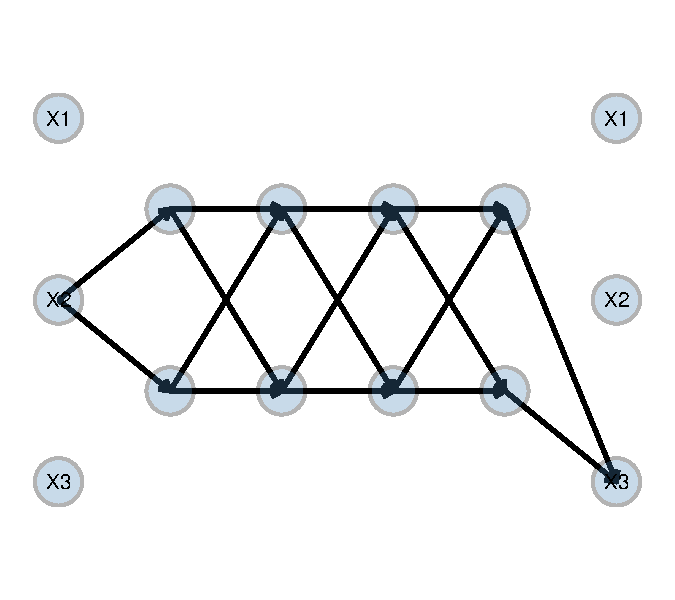
\includegraphics[width=0.5\linewidth]{img/exp1_CS.pdf}
\caption{Neural network architecture for the complex shift on $X_3$ from $X_2$. The complex shift is modeled by a neural network with 4 hidden layers of shape (2, 2, 2, 2), using non-linear activation functions (sigmoid).}
\label{fig:exp1_CS}
\end{figure}




\textbf{Model evaluation: } We compare the estimated intercepts, learned coefficients, and the complex shift to the true values used in the DGP. We also compare the sampled observational and interventional distributions to the true distributions. For the counterfactual queries, we show the estimated counterfactual values for $X_2$ under an intervention on $X_1$ at a specific value, and compare these to the true counterfactual outcomes.




\section{Experiment 2: ITE on International Stroke Trial (IST)} \label{sec:methods_experiment2}


% describe the data of stroke trial https://pubmed.ncbi.nlm.nih.gov/9174558/
% Results on IST trial with the interpretation in the discussion part.

%  here the authors made the IST database available and described the trial, we downloaded the CSV
% https://trialsjournal.biomedcentral.com/articles/10.1186/1745-6215-12-101 


% Results: The IST dataset includes data on 19 435 patients with acute stroke, with 99% complete follow-up. Over 26.4% patients were aged over 80 years at study entry. Background stroke care was limited and none of the patients received thrombolytic therapy.
% 
% 
\citet{chen2025} evaluated multiple causal ML methods on the International Stroke Trial (IST), to estimate the individualized treatment effects. They demonstrated that none of the applied ML methods generalized well, as performance on the test data differed significantly from the training data on the chosen evaluation metrics.
In this experiment, we replicate the analysis on the same data by applying three causal ML methods for ITE estimation, to investigate whether we obtain similar results as the authors.


\medskip

\textbf{Data:} The International Stroke Trial was a large, randomized controlled trial conducted in the 1990s to assess the efficacy and safety of early antithrombotic treatment in patients with acute ischemic stroke \citep{IST1997}. Using a 2x2 factorial design, 19,435 patients across 36 countries were randomized within 48 hours of symptom onset to receive aspirin, subcutaneous heparin, both, or neither. Patients allocated to aspirin (300 mg daily for 14 days) had a 6-month death or dependency rate of 62.2\%, compared to 63.5\% in the control group not receiving aspirin, corresponding to a statistically significant absolute risk reduction after adjustment for baseline prognosis (1.4\%, p = 0.03). The authors stated that there was no interaction between aspirin and heparin in the main outcomes. In this thesis, we focus exclusively on the aspirin vs. no aspirin comparison and the outcome of death or dependency at 6 months after stroke.

The dataset used in this experiment was made publicly available by \citet{sandercock2011} and contains individual-level data, including baseline covariates assessed at randomization, treatment allocation, and 6-month outcomes, with a follow-up rate of 99\%.

We used the same data pre-processing steps as \citet{chen2025} to ensure comparability of results. 5.9\% of individuals had incomplete data and were removed from the dataset. We used 2/3 of the data for fitting the models and 1/3 as a hold out test set. The final dataset included 21 baseline variables recorded at randomization: aspirin allocation (treatment), age, delay between stroke and randomization (in hours), systolic blood pressure, sex, CT performed before randomization, visible infarct on CT, atrial fibrillation, aspirin use within 3 days prior to randomization, and presence or absence of neurological deficits (including face, arm/hand, leg/foot deficits, dysphasia, hemianopia, visuospatial disorder, brainstem or cerebellar signs, and other neurological deficits), as well as consciousness level, stroke subtype, and geographical region. The outcome variable was death or dependence at 6 months.


\medskip

\textbf{Models for ITE estimation: } The aim is to estimate the ITE based on baseline characteristics. As a benchmark, we apply a T-learner logistic regression (following \citet{chen2025}, using the \texttt{stats} package). As a more complex model, we apply a T-learner tuned random forest (using the \texttt{comets} package \citep{comets}), which tunes the number of variables considered for splitting at each node (\texttt{mtry}) and the maximum tree depth (\texttt{max.depth}) using out-of-bag error, with 500 trees. Additionally, we apply an S-learner TRAM-DAG. For the random forest and TRAM-DAG based methods, we additionally scale numerical and dummy encode categorical covariates prior to model training. The transformation function of the outcome is modelled by a complex intercept $h(Y \mid T, \mathbf{X}) = CI(T, \mathbf{X})$, with 4 hidden layers of shape (20, 10, 10, 2). This architecture allows for interaction between the treatment and covariates. Furthermore, batch normalization, ReLU activation, and dropout (0.1) are applied to prevent overfitting and stabilize learning. A validation set comprising 20\% of the training data is used to select the model with the lowest out-of-sample negative log-likelihood, while the test set remains untouched for final evaluation. Since the IST stroke trial is a randomized controlled trial, the full potential of TRAM-DAGs (that lies in the observational setting) is not needed, as only the outcome has to be modelled as a function of the baseline patient characteristics. Nevertheless, this is not a reason not to apply it.


\medskip

\textbf{Model evaluation: } For validation, since the ground truth is not known, we first rely on calibration plots to assess the general prediction power for the probabilities. Second, we predict the potential outcomes with the trained models to estimate the ITE on the training and test set in terms of the risk difference $\text{ITE}_i = \text{P}(Y_i=1|T=1, \mathbf{X}_i) - \text{P}(Y_i=1|T=0, \mathbf{X}_i)$. For visual validation, we show the densities of the estimated ITEs on both datasets, and the ITE-ATE plots to assess whether the estimated ITEs align with the observed outcomes.










% possible example of unobserved interaction:
% An example could be the psychological condition of a patient which might also affect how the treatment works, this is not a confounder but an effect modifier, and i would assume that this variable is rarely recorede or measured.






\section{Experiment 3: ITE model robustness in RCTs (simulation)} \label{sec:methods_experiment3}

In this section, we perform a simulation study to estimate the ITE using different models in an RCT setting under various scenarios. The aim is to identify conditions under which ITE estimation fails, and whether such failure is model-agnostic -- i.e., driven by external factors such as unobserved covariates or the strength of the treatment effect, rather than by the model class itself. This may provide insight into why ITE estimation can fail in real-world applications, as demonstrated by \citet{chen2025} on the IST dataset and replicated in our own work in Experiment 2 (Section~\ref{sec:results_experiment2}). The simulation is based on a data-generating process (DGP) that resembles an RCT. We assume a binary outcome and a set of covariates that influence the outcome. There may also be treatment-covariate interactions that are responsible for heterogeneity in the treatment effect.

\medskip

\textbf{Data-generating process:} Data is generated similarly to the approach proposed by \citet{hoogland2021}. The binary treatment ($T$) is sampled from a Bernoulli distribution with probability 0.5. The five covariates ($\mathbf{X}$), representing patient-specific characteristics at baseline, are drawn from a multivariate standard normal distribution with a compound symmetric covariance matrix ($\rho=0.1$). The binary outcome ($Y$) is sampled from a Bernoulli distribution with probability $\text{P}(Y_i = 1 \mid  \mathbf{X_i} = \mathbf{x_i}, T_i = t_i) = \text{logit}^{-1} \left(\beta_0 + \beta_T t_i + \boldsymbol{\beta}_X^\top \mathbf{x_i} + t_i \cdot \boldsymbol{\beta}_{TX}^\top \mathbf{x_{TX,i}} \right)$, where $i$ denotes the patient index, and $\mathbf{x}_{TX,i}$ denotes the subset of covariates that interact with the treatment.

The simulated datasets are generated under three scenarios, where coefficients are set to different values or not all variables are observed. In Scenario 1, the coefficients are: $\beta_0 = 0.45$ (intercept), $\beta_T = -0.85$ (direct treatment effect), $\boldsymbol{\beta}_X = (-0.5, 0.8, 0.2, 0.6, -0.4)$ (direct covariate effects), and $\boldsymbol{\beta}_{TX} = (0.9, 0.1)$ (interaction effects between treatment and covariates $X_1$ and $X_2$ on the outcome). In Scenario 2, the same coefficients are used, but the covariate $X_1$, which is responsible for a large portion of the heterogeneity, is not observed in the final dataset. This is expected to cause difficulties in estimating the ITE. In Scenario 3, the coefficients for the direct treatment and interaction effects are set to $\beta_T = -0.05$ and $\boldsymbol{\beta}_{TX} = (-0.01, 0.03)$ to represent a weak treatment effect and low heterogeneity. All other coefficients remain unchanged, and all covariates are observed. The DAGs corresponding to the three scenarios are presented in Figure~\ref{fig:simulation_dags}.


% here include 3 figures side by side 
% /img/results_ITE_simulation/simulation_observed.png
% simulation_unobserved.png
% simulation_small_effects.png

\begin{figure}[H]
\centering
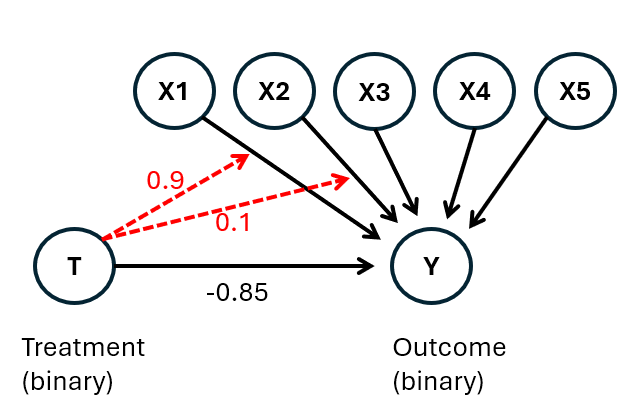
\includegraphics[width=0.3\textwidth]{img/results_ITE_simulation/simulation_observed.png}
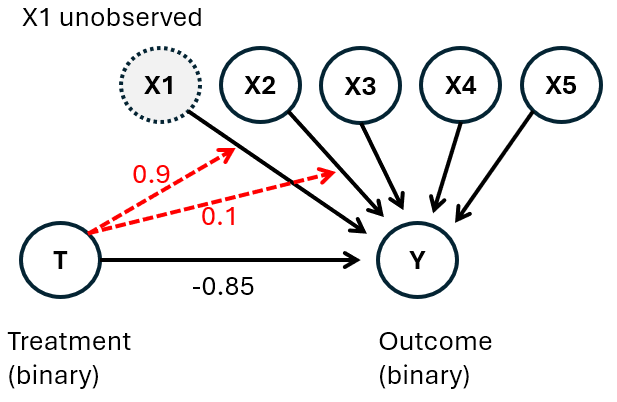
\includegraphics[width=0.3\textwidth]{img/results_ITE_simulation/simulation_unobserved.png}
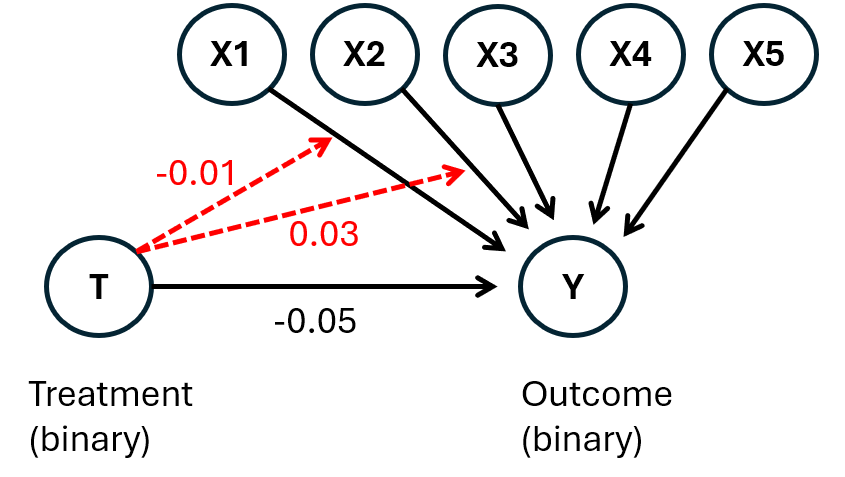
\includegraphics[width=0.3\textwidth]{img/results_ITE_simulation/simulation_small_effects.png}
\caption{Data-generating process (DGP) for the three scenarios in the ITE simulation study (RCT). Interaction effects between treatment ($T$) and covariates ($X_1$ and $X_2$) on the outcome ($Y$) are shown in red. Left: Scenario 1, where all covariates are observed and both treatment effect and heterogeneity are strong; Middle: Scenario 2, with the same DGP as in Scenario 1, but where covariate $X_1$ is not observed; Right: Scenario 3, where the treatment effect and heterogeneity are weak, and all covariates are observed.}
\label{fig:simulation_dags}
\end{figure}




% The data is generated for three different scenarios, where the coefficients are set to different values to represent different treatment effects and interaction effects and by removing the covariate $X1$ from the final dataset in scenario 2, hence making it unobserved. The scenarios are summarized in Table \ref{tab:simulation_scenarios}.


% Table with szenarios:

% Szenario 1: 
% description: strong direct and interaction effect of treatment, fully observed
% coefficients: \beta_0 = 0.45, \beta_T = -0.85,  \boldsymbol{\beta}_X = c(-0.5, 0.8, 0.2, 0.6, -0.4), \boldsymbol{\beta}_{TX} = c(0.9, 0.1)
% motivation: this scenario should represent the ideal case where there is high heterogeneity and all variables are observed, hence the ITE estimation is assumed to work well.

% Szenario 2:
% description: strong direct and interaction effect of treatment, but covariate X1 not observed
% coefficients: \beta_0 = 0.45, \beta_T = -0.85,  \boldsymbol{\beta}_X = c(-0.5, 0.8, 0.2, 0.6, -0.4), \boldsymbol{\beta}_{TX} = c(0.9, 0.1)
% motivation: removing the covariate X1, which is responsible for much of the heterogeneity, should cause difficulties in ITE estimation because the heterogeneity can not be attributed to the right covariate.

% Szenario 3:
% description: weak direct and interaction effect of treatment, fully observed
% coefficients: \beta_0 = 0.45, \beta_T = -0.05,  \boldsymbol{\beta}_X = c(-0.5, 0.8, 0.2, 0.6, -0.4), \boldsymbol{\beta}_{TX} = c(-0.01, 0.03)
% motivation: this scenario should represent the case where the treatment effect is weak and heterogeneity is low, hence the model should estimate only small range of ITE.





% \subsubsection*{Scenario 1: Strong effects, all covariates observed}
% 
% This scenario represents an ideal case in which the treatment has a strong direct and interaction effect. All covariates are observed, supposedly enabling effective ITE estimation. The coefficients are set as follows:
% 
% 
% 
% % X1 and X2 interact with treatment
% \begin{align*}
%     \beta_0 &= 0.45,\quad \beta_T = -0.85, \\
%     \boldsymbol{\beta}_X &= (-0.5,\ 0.8,\ 0.2,\ 0.6,\ -0.4), \\
%     \boldsymbol{\beta}_{TX} &= (0.9,\ 0.1) , X_1 \text{ and } X_2 \text{ interact with treatment}
% \end{align*}
% 
% \vspace{0.5em}
% 
% \subsubsection*{Scenario 2: Strong effects, covariate \boldmath$X_1$ unobserved}
% 
% This scenario uses the same coefficients as Scenario 1, but with covariate $X_1$ removed from the dataset. As $X_1$ drives a large portion of the treatment effect heterogeneity, the estimation of the ITE is expected to be biased or incomplete when $X_1$ is not observed.
% 
% 
% \begin{align*}
%     \beta_0 &= 0.45,\quad \beta_T = -0.85, \\
%     \boldsymbol{\beta}_X &= (-0.5,\ 0.8,\ 0.2,\ 0.6,\ -0.4), \\
%     \boldsymbol{\beta}_{TX} &= (0.9,\ 0.1) , X_1 \text{ and } X_2 \text{ interact with treatment}
% \end{align*}
% \textit{Note: $X_1$ is not included in the final dataset.}
% 
% \vspace{0.5em}
% 
% \subsubsection*{Scenario 3: Weak Effects, All Covariates Observed}
% 
% This scenario illustrates a setting with minimal treatment effect and weak treatment-covariate interaction. While all covariates are observed, the model is expected to recover only low-variance ITEs due to limited signal.
% 
% \begin{align*}
%     \beta_0 &= 0.45,\quad \beta_T = -0.05, \\
%     \boldsymbol{\beta}_X &= (-0.5,\ 0.8,\ 0.2,\ 0.6,\ -0.4), \\
%     \boldsymbol{\beta}_{TX} &= (-0.01,\ 0.03), X_1 \text{ and } X_2 \text{ (weakly) interact with treatment}
% \end{align*}


\textbf{Models for ITE estimation:} The datasets generated from the DGP under the three scenarios are used to estimate the ITE using different models. We applied the following models: T-learner logistic regression (\texttt{stats} package), T-learner logistic lasso regression (\texttt{glmnet} package \citep{friedman2010}, with the regularization parameter $\lambda$ estimated via 10-fold cross-validation), S-learner logistic lasso regression (same as the T-learner), T-learner random forest (\texttt{randomForest} package \citep{breiman2001}, 100 trees), and T-learner tuned random forest (\texttt{comets} package \citep{comets}, which tunes the number of variables considered for splitting at each node (\texttt{mtry}) and the maximum tree depth (\texttt{max.depth}) using out-of-bag error, 500 trees). 

While all models were applied, we present only the results of the T-learner logistic regression as a benchmark (same model as used in the data-generating process), and the tuned random forest as representation of a complex non-parametric model. In Appendix~\ref{sec:default_rf_ite}, we additionally present the results for a standard random forest evaluated for Scenario 1 to illustrate the importance of model tuning to prevent overfitting and ensure accurate calibration.

All models were trained on a training set and evaluated on a test set, each consisting of 10,000 samples generated from the same DGP. TRAM-DAGs would also be well suited for ITE estimation in this setting, but we chose not to apply them in this experiment, since the main objective is to assess behavioral differences between complex and simple models under different scenarios. TRAM-DAGs are applied in other experiments in this thesis.

\medskip

\textbf{Model evaluation:} Model performance is evaluated visually on both the training and test datasets. For predictive performance, we present true vs. predicted probabilities $\text{P}(Y = 1 \mid X, T)$ to assess how well each model is calibrated. Plots of true vs. predicted ITEs show how closely the model estimates match the true effects. Since the true probabilities and ITEs are known by design in this simulation, direct evaluation of calibration and prediction accuracy is possible, unlike in real-world applications.

To assess whether estimated ITEs correspond to actual observed outcomes, we use ITE-ATE plots. These show the observed average treatment effect (ATE), calculated as $\text{P}(Y = 1 \mid T = 1) - \text{P}(Y = 1 \mid T = 0)$, in the respective subgroups of estimated ITEs. Accurate models should produce ITE-ATE points that align with the identity line.

These simulation scenarios allow us to assess ITE estimation performance under challenging conditions such as omitted variables and weak treatment effects. The subsequent results reveal which models remain robust under such violations and provide insight into possible real-world estimation failures.








% quantile treatment effect
% Papers:

% https://journals.sagepub.com/doi/pdf/10.1177/1536867X1001000309
% https://epge.fgv.br/files/1125.pdf


\section{Experiment 4: ITE estimation with TRAM-DAGs (simulation)} \label{sec:methods_experiment4}


We claim that the TRAM-DAG framework can be effectively used for ITE estimation on observational data with confounding and mediating variables, provided that the identifiability assumptions are satisfied and the DAG is fully known. Therefor, we apply TRAM-DAGs in both a confounded and a randomized setting, using data simulated according to the DAGs shown in Figure~\ref{fig:ite_dag_observational}. The binary treatment ($X_4$) is the intervention variable, and the goal is to estimate the ITE for the continuous outcome $Y$.


\begin{figure}[H]
\centering
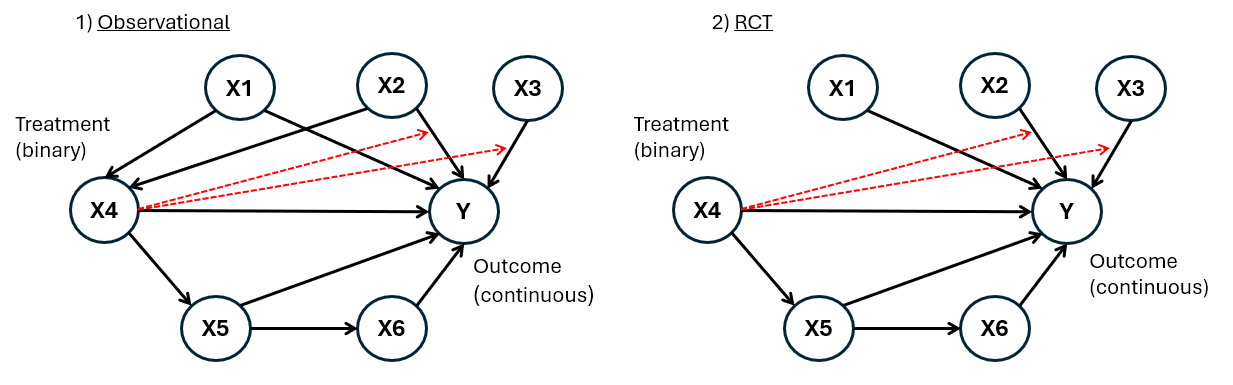
\includegraphics[width=0.85\textwidth]{img/exp4_dags.png}
\caption{DAGs used for the simulation to estimate the ITE. Left: observational; Right: RCT setting. The source nodes $X_1$, $X_2$, and $X_3$ come from a multivariate standard normal distribution ($\rho=0.1$). In the observational setting, the binary treatment $X_4$ depends on the parents $X_1$ and $X_2$. In the RCT setting, this dependency is omitted due to randomization. The outcome $Y$ depends on all variables, with additional interaction effects between the treatment and the variables $X_2$ and $X_3$. All variables except the treatment $X_4$ are continuous.}
\label{fig:ite_dag_observational}
\end{figure}

\medskip

\textbf{Illustrative scenario:} An possible real-world scenario that follows the structure of the proposed DAG could be the following: A marketing campaign is conducted to increase customer spending. The treatment is the marketing email ($X_4$) sent to customers. If the treatment is not randomized, it depends on prior total spend ($X_1$) and the customer engagement score ($X_2$). The outcome is the total spend in the 30 days following the email, denoted as $Y$. The prior total spend ($X_1$) and customer engagement score ($X_2$) act as confounders, influencing both the treatment and the outcome. The customer satisfaction score ($X_3$), obtained from a recent survey, is another predictor. The time spent on the website after receiving the email ($X_5$) is a mediator that affects the number of product pages viewed ($X_6$), which in turn influences the total spend ($Y$). Interaction effects exist between the treatment ($X_4$) and both $X_2$ and $X_3$, meaning the treatment effect differs based on the customer's engagement and satisfaction levels. The goal is to estimate the individualized treatment effect (ITE) of the marketing email ($X_4$) on the total spend ($Y$), in order to personalize customer targeting.

\medskip

\textbf{Data-generating process:} The standard logistic distribution was chosen as the noise distribution to align with other examples in this thesis. Any other noise distribution could also be used here, as we are not interested in coefficient interpretability in this experiment. All variables except the binary treatment $X_4$ are continuous. The source nodes $X_1$, $X_2$, and $X_3$ are generated from a multivariate standard normal distribution with a compound symmetric covariance matrix ($\rho = 0.1$). These variables represent baseline patient characteristics.

In the observational setting, $X_1$ and $X_2$ act as confounders by influencing both the treatment assignment $X_4$ and the outcome $Y$. In the RCT setting, these dependencies are removed due to randomization. The mediator $X_5$ depends on treatment $X_4$, and $X_6$ depends on $X_5$. The log-odds of the continuous outcome $Y$ depend linearly on all covariates, including additional interaction terms between the treatment and $X_2$ and $X_3$. Equation~\ref{eq:outcome_dgp} defines the outcome on the log-odds scale:

\begin{equation}
h(y \mid \mathbf{X}) = h_I(y) + \boldsymbol{\beta}_X^\top \mathbf{X} + X_4 \cdot (\boldsymbol{\beta}_{TX}^\top \mathbf{X}_{\text{TX}})
\label{eq:outcome_dgp}
\end{equation}

Here, $h_I(y)$ is the intercept function, $\mathbf{X}$ is the full covariate vector, and $\mathbf{X}_{\text{TX}} = \{X_2, X_3\}$ denotes the interaction covariates that affect the outcome only when treatment is applied ($X_4 = 1$). The intercept function $h_I(y)$ must be smooth and monotonically increasing. We define it as $h_I(y) = \tan(y/2) / 0.2$ for $y \in [-2, 2]$, and extrapolate linearly at the boundaries.

The coefficients are set as $\boldsymbol{\beta}_X = (-0.5,\ 0.5,\ 0.2,\ 1.5,\ -0.6,\ 0.4)$, where the value $1.5$ represents the direct effect of treatment $X_4$ on the outcome. The interaction coefficients are set to $\boldsymbol{\beta}_{TX} = (-0.9,\ 0.7)$.

\medskip

\textbf{Three scenarios:} The experiment is conducted under three different scenarios regarding the effect of the treatment on the outcome $Y$ in the DGP: (1) both direct and interaction effects, (2) only a direct effect, and (3) only interaction effects. Depending on the scenario, the corresponding coefficients in $\boldsymbol{\beta}_X$ and $\boldsymbol{\beta}_{TX}$ are set to zero.

\medskip


\textbf{TRAM-DAG estimation:} In both the observational and RCT settings, the TRAM-DAG is fitted as an S-learner (i.e., a single model including the treatment variable). To allow for full flexibility, all nodes with parents are modeled using complex intercepts with three hidden layers of size (10, 10, 10), without batch normalization or dropout, unsing ReLU activation. The model is trained on a dataset of 20,000 samples. To prevent overfitting, an additional validation set of 10,000 samples is used, and the final model is selected using early stopping based on validation loss.

\medskip

\textbf{ITE estimation procedure:} In contrast to most of the research we analyzed, where the ITEs are typically defined in terms of expected values of the potential outcomes, here we estimate the quantile treatment effect (QTE), specifically at the median. For each individual, we calculate the difference between the 0.5-quantiles of the potential outcome distributions under treatment and control. \citet{chernozhukov2005}, for example, highlighted the ability of quantile regression models in heterogeneous treatment effect estimation. QTEs are particularly relevant when the distributional behavior of outcomes beyond the mean is of interest. The median QTE is defined as

\begin{equation}
\text{QTE}^{(0.5)}(\mathbf{x}) = Q_{Y(1) \mid \mathbf{X} = \mathbf{x}}(0.5) - Q_{Y(0) \mid \mathbf{X} = \mathbf{x}}(0.5),
\end{equation}


where $Q_{Y(t) \mid \mathbf{X} = \mathbf{x}}(q)$ denotes the $q$-th quantile of the potential outcome distribution under treatment $t$.

Once the TRAM-DAG model is fitted on observed data, we can access the inverse transformation functions $X_i = h^{-1}(Z_i \mid \text{pa}(X_i))$, which represent the structural equations of the DAG. ITE estimation proceeds in three steps, according to Algorithm~\ref{alg:ite_qte}. First, the latent values $z_{ij}$ for the explanatory variables $X_i \in \{X_1, X_2, X_3, X_5, X_6\}$ are computed for each sample $j$ using the transformation functions conditioned on their observed parents. Second, the treatment variable $X_4$ is intervened on using the do-operator for both $X_4 = 0$ and $X_4 = 1$. For each of these two treatment states, $X_5$, $X_6$, and the potential outcome (distribution) $Y$ are sampled sequentially using the latent encodings and inverse transformations. This means that the counterfactuals for $X_5$ and $X_6$ are determined. This results in two potential outcome distributions per individual, as illustrated in Figure~\ref{fig:exp4_potential_outcomes}. Finally, for each individual, the median is determined for both potential outcome distributions and the QTE is calculated as the difference between the two medians. Note that estimating the potential outcomes in terms of expected values would also be possible -- either by repeatedly sampling from each outcome distribution or, potentially, by numerical integration. However, for this experiment, we chose to estimate the QTE. For simplicity, we will refer to these as ITEs throughout the remainder of the experiment.


\begin{figure}[H]
\centering
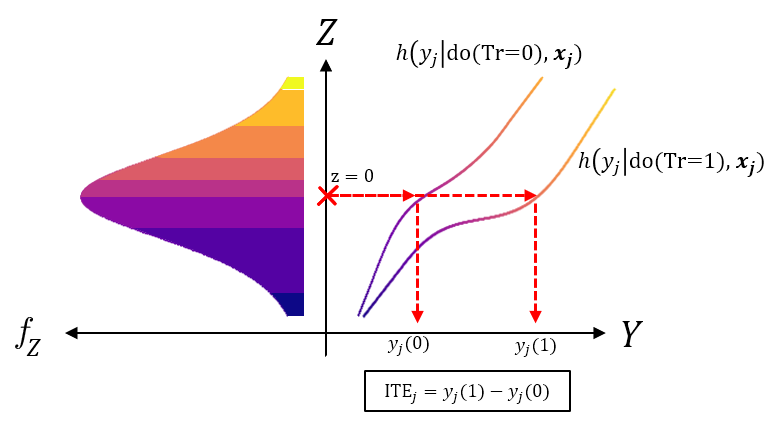
\includegraphics[width=0.6\textwidth]{img/potential_outcomes_y.png}
\caption{ITE estimation in terms of quantile treatment effect (QTE) at the median with TRAM-DAGs. The two transformation functions represent the distributions of the potential outcomes under both treatments. For the QTE(0.5), the median of the latent distribution (0 for the standard logistic) is evaluated on both transformation functions to determine the median potential outcomes. We define the ITE for an individual as the difference of the median potential outcomes.}
\label{fig:exp4_potential_outcomes}
\end{figure}


\begin{algorithm}
\caption{ITE estimation (QTE) using TRAM-DAGs}
\label{alg:ite_qte}
\begin{algorithmic}
\State \textbf{Input:} Fitted TRAM-DAG, dataset of $n$ individuals
\For{each individual $j = 1$ to $n$}
  \State \textbf{Step 1: Determine latent values}
  \For{each explanatory node $X_i \in \{X_1, X_2, X_3, X_5, X_6\}$}
    \State Compute latent value: $z_{ij} = h_i(x_{ij} \mid \text{pa}(x_{ij}))$
  \EndFor

  \State \textbf{Step 2: Generate potential outcomes under treatment and control}
  \For{$x_4 \in \{0, 1\}$} \Comment{Simulate both treatment states}
    \State Fix $X_4 = x_4$ (intervention)
    \State Sample $X_5$ and $X_6$ sequentially using $z_{ij}$ and inverse transformations
    \State Sample potential outcome $y_j(x_4)$ using $z_{7,j} = 0$ (median of the potential outcome distribution)

  \EndFor

  \State \textbf{Step 3: Compute ITE (QTE) for individual $j$}
  \State $\text{ITE}_j = y_j(1) - y_j(0)$  %\text{median}(y_j(1)) - \text{median}(y_j(0))$
\EndFor
\State \textbf{Output:} ITE estimates $\{\text{ITE}_j\}_{j=1}^n$
\end{algorithmic}
\end{algorithm}


\medskip

\textbf{Model evaluation:} Validation is conducted on the training dataset and on an independent test dataset of same size. During the data-generating process, the true potential outcomes under both treatment states were recorded for each individual, which allows for exact computation of the true ITE. The estimated ITEs are evaluated against the true values using several visual and numerical metrics. These include density plots of the estimated ITEs, scatter plots of true vs. estimated ITEs, and ITE-ATE plots where the observed ATE per ITE subgroup is computed as the difference in medians. In addition, the average of the estimated ITEs is compared to the true average ITE and to the empirical ATE from the RCT setting. The scatter plot of true versus estimated ITEs is the most informative validation, as it directly reflects how accurately the model estimated ITEs.














% 
% \textbf{ITE estimation procedure: } In contrast to the potential outcomes framework, where the potential outcomes are defined as the expected value of the outcome under treatment, we define the potential outcomes as the median of the outcome distribution under treatment - the quantile treatment effect (QTE). For simplicity, we will further refer to the individual treatment effect as ITE even though technically, the QTE is meant. Determining the potential outcomes in terms of the expected values would also be possible, but would require us to repeatedly sample from each resulting potential outcome distribution for each individual and average the results. This was computationally too time consuming and therefore we decided to estimate the QTE instead. In the ITE estimation in the previous examples with binary outcome, this was not necessary, since the potential outcomes were defined as the probabilities of the outcome under treatment and control, hence a single number that represents the expected value.
% 
% Notes after Meeting 24.06.25: Depending on the problem, CATE in terms of expected values of potential outcomes might be more appropriate than QTE, but also QTE could be better. Depends. If we wanted the potential outcomes based on the expected values, we have two options. either sample latent values and evaluate inverse tranformation functions. from those two sample distributions calculate the means to get the expected potential outcomes. Lucas suggested that we could also use numerical integreation instead, then we would not have to sample.
% 
% In contrast to the mean-based estimands above, the quantile treatment effect (QTE) evaluates differences in the distribution of potential outcomes. For instance, the median treatment effect is defined as
% 
% \citep{chernozhukov2005} also wrote about QTE (also in the context of instrumental variables). (also says to can deal with unobserved heterogeneity.. although, probably only as extension of our approach)
% 
% \begin{equation}
% \tau^{(0.5)}(x) = Q_{Y(1) \mid X = x}(0.5) - Q_{Y(0) \mid X = x}(0.5),
% \end{equation}
% 
% where $Q_{Y(t) \mid X = x}(q)$ denotes the $q$-th quantile of the potential outcome under treatment $t$. QTEs are particularly relevant when treatment effects are not symmetrically distributed or when tail behavior is of interest. In experiment 4, Section \ref{sec:methods_experiment4} we performed a simulation study using the median for the QTE estimation.
% 
% Once the TRAM-DAG is fitted, we obtained the estimated (inverse) transformation functions $X_i = h^{-1}(Z_i \mid pa(X_i))$ that represent the equations $X_i = f(Z_i, pa(X_i))$ in the structural causal model. The process for the ITE estimation is outlined in \ref{alg:ite_qte}. It is done as follows: In a first step to estimate the ITE, we determine the latent values $z_{ij}$ in all observed samples $j$ for the explanatory nodes $i$ - X1, X2, X3, X5 and X6. The latent values are the values of the transformation functions at the observed value of the variable given the observed values of its parents $z_{ij} = h_i(x_{ij} \mid pa(x_{ij}))$. In a second step, these latent values $z_{ij}$ are used to sequentially sample from the two interventional distributions when setting the treatment X4 to either 0 or 1. For each individual, these interventions impact the mediator nodes X5 and X6 as well as the outcome Y. The source nodes X1, X2 and X3 remain equal under both treatments. The treatment X4 is the variable which we fix by the do-intervention. X5 and X6 will change according to the treatment. Finally, for each set of samples $j$ (meaning for each individual) we get two distributions for the outcome, one under treatment and one under control. Then, for each individual, we calculate the iTE as the difference between the medians of the potential outcome distributions under treatment and control, as visualized in Figure~\ref{fig:exp4_potential_outcomes}.
% 
% 
% 
% 
% \begin{figure}[H]
% \centering
% 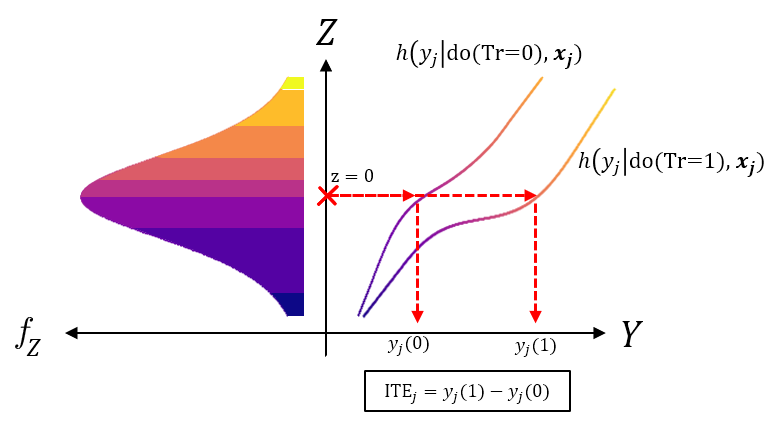
\includegraphics[width=0.6\textwidth]{img/potential_outcomes_y.png}
% \caption{Quantile treatment effect (QTE) at the median with TRAM-DAGs. The two transformation functions represent the distributions of the potential outcomes under both treatmetns. For the QTE(0.5), the median of the latent distribution is evaluated on both transformation functions to determine the median-potential-ouotcomes. This is in contrast to the ITE based on the expected values of the potential outcomes.}
% \label{fig:exp4_potential_outcomes}
% \end{figure}
% 
% 
% 
% 
% \begin{algorithm}
% \caption{ITE Estimation (QTE) Using TRAM-DAG in Observational Data}
% \label{alg:ite_qte}
% \begin{algorithmic}[1]
% \State \textbf{Input:} Fitted TRAM-DAG, observational dataset with $n$ samples
% \For{each sample $j = 1$ to $n$}
%   \State \textbf{Step 1: Encode explanatory nodes}
%   \For{each explanatory node $X_i \in \{X_1, X_2, X_3, X_5, X_6\}$}
%     \State Compute latent value: $z_{ij} = h_i(x_{ij} \mid \text{pa}(x_{ij}))$
%   \EndFor
% 
%   \State \textbf{Step 2: Generate potential outcomes under treatment and control}
%   \For{$x_4 \in \{0, 1\}$} \Comment{Simulate both treatment states}
%     \State Fix $X_4 = x_4$ (intervention)
%     \State Sample $X_5$ and $X_6$ sequentially using $z_{ij}$ and inverse transformations
%     \State Sample potential outcome $y_j^{(x_4)}$ using $z_{7,i} = 0$ (median of the potential outcome distribution)
% 
%   \EndFor
% 
%   \State \textbf{Step 3: Compute QTE for individual $j$}
%   \State $\text{ITE}_j = \text{median}(y_j^{(1)}) - \text{median}(y_j^{(0)})$
% \EndFor
% \State \textbf{Output:} ITE estimates $\{\text{ITE}_j\}_{j=1}^n$
% \end{algorithmic}
% \end{algorithm}
% 
% 
% 
% 
% 
% \textbf{Validation of results: } In the data generating mechanism, along with the actually sampled values, the potential values under both treatments are also recorded and used to determine the true QTE (the ITE based on the 50 percent quantiles of the potential outcome distributions of each individual.)
% The results are displayed by densities of the estimated ITE, the scatterplots of the true vs. estimated ITE, the ITE-ATE plot with the difference in medians as ATE within subgroups to make it comparable to the estimated ITEs. Furthermore the average of all estimated and true (dgp) ITEs are presented in table format. We further calculate the ATE as the overall difference in medians in the RCT setting and compare it to the estimated values based on the ITEs, althogh if this comparison in terms of the mean of a difference in medians is valid we did not further proof. It should be rather regarded as information, but not as proof. The scatterplot of the true vs. estimated ITE poses the most important validation.


% Check if true? probably not entirely... in both, the RCT and in the Observational setting, also other models could be applied instead of TRAM-DAG. As long as all confounders are included in the model, we controll for the confounders and can get unbiased results. For example a T-learner Colr($Y \sim X_1 + X_2 + X_3$) (because Colr is basically what we did in the DGP) fitted on both treatment groups separately could be used to estimate the ITE in our proposed experiment. This might only be possible so easily as long as we do not assume additional interactions between the treatment and the mediators $X_5$ and $X_6$. If we would assume such interactions, we would have to include these in the model as well, which would make it more complex and possibliy requires to fit and apply multiple models. If there are no interactions with the mediators, they can be omitted, since we are interested in the total treatment effects and not in separating the effect (mediation analysis). But again, we can only omit if these variables do not contain additional information about treatment effect heterogeneity. The reasoning is because to estimate the total effect one should not control for mediators. (check if really true!!!)  However, the TRAM-DAG framework is well suited to also deal with mediators and calculate counterfactuals, therefore we think it is a good example to show its capabilities.


% Notes after Meeting 24.06.25: Depending on the problem, CATE in terms of expected values of potential outcomes might be more appropriate than QTE, but also QTE could be better. Depends. If we wanted the potential outcomes based on the expected values, we have two options. either sample latent values and evaluate inverse tranformation functions. from those two sample distributions calculate the means to get the expected potential outcomes. Lucas suggested that we could also use numerical integreation instead, then we would not have to sample.




\section{Software}


All code used in this thesis is available on GitHub: \url{https://github.com/mikekr97/MA_Mike}.

All analyses were conducted in R~\citep{R} (version 4.4.2) using RStudio. The packages \texttt{keras}~\citep{keras} (version 2.15.0), \texttt{tensorflow}~\citep{tensorflow} (version 2.16.0), and \texttt{reticulate}~\citep{reticulate} (version 1.40.0) were used to build and train neural networks through Python's TensorFlow backend. These tools allowed for the use of deep learning methods directly within the R environment.


% Maybe it is the methods section. Here however, we give a couple hints.
% Note that you can wisely use \rr{preamble}-chunks. Minimal, is likely:
% 
% 
% \bigskip
% 
% \hrule
% <<echo=TRUE>>=
% library(knitr)
% opts_chunk$set(
%     fig.path='figure/ch02_fig',
%     self.contained=FALSE,
%     cache=TRUE
% )
% @
% \hrule
% 
% \bigskip
% 
% Defining figure options is very helpful:
% 
% 
% \bigskip
% 
% 
% \hrule
% <<echo=TRUE,cache=FALSE>>=
% library(knitr)
% opts_chunk$set(fig.path='figure/ch02_fig',
%                echo=TRUE, message=FALSE,
%                fig.width=8, fig.height=2.5,
%                out.width='\\textwidth-3cm',
%                message=FALSE, fig.align='center',
%                background="gray98", tidy=FALSE, #tidy.opts=list(width.cutoff=60),
%                cache=TRUE
% )
% options(width=74)
% @
% \hrule
% 
% \bigskip
% 
% This options are best placed in the main document at the beginning. Otherwise a \verb+cache=FALSE+ as knitr option is necessary to overrule a possible  \verb+cache=TRUE+ flag.
% 
% \bigskip
% 
% Notice how in Figure~\ref{f02:1} everything is properly scaled.
% 
% \begin{figure}
% <<echo=FALSE>>=
% par(mai=c(.8,.8,.1,.1))
% set.seed(12)
% plot( runif(30), type='l')
% @
%   \caption{Test figure to illustrate figure options used by knitr.}
%   \label{f02:1}
% \end{figure}
% 
% 
% \section{Citations}
% 
% Recall the difference between \verb+\citet{}+ (e.g., \citet{Chu:Geor:99}), \verb+\citep{}+ (e.g., \citep{Chu:Geor:99}) and \verb+\citealp{}+ (e.g., \citealp{Chu:Geor:99}).
% For simplicity, we include here all references in the file \verb+biblio.bib+ with the command \verb+\nocite{*}+.\nocite{*}

